% Options for packages loaded elsewhere
\PassOptionsToPackage{unicode}{hyperref}
\PassOptionsToPackage{hyphens}{url}
\PassOptionsToPackage{dvipsnames,svgnames,x11names}{xcolor}
%
\documentclass[
  10pt,
  a4paper,
  numbers=noendperiod,
  DIV=9]{scrartcl}

\usepackage{amsmath,amssymb}
\usepackage{iftex}
\ifPDFTeX
  \usepackage[T1]{fontenc}
  \usepackage[utf8]{inputenc}
  \usepackage{textcomp} % provide euro and other symbols
\else % if luatex or xetex
  \usepackage{unicode-math}
  \defaultfontfeatures{Scale=MatchLowercase}
  \defaultfontfeatures[\rmfamily]{Ligatures=TeX,Scale=1}
\fi
\usepackage{lmodern}
\ifPDFTeX\else  
    % xetex/luatex font selection
\fi
% Use upquote if available, for straight quotes in verbatim environments
\IfFileExists{upquote.sty}{\usepackage{upquote}}{}
\IfFileExists{microtype.sty}{% use microtype if available
  \usepackage[]{microtype}
  \UseMicrotypeSet[protrusion]{basicmath} % disable protrusion for tt fonts
}{}
\makeatletter
\@ifundefined{KOMAClassName}{% if non-KOMA class
  \IfFileExists{parskip.sty}{%
    \usepackage{parskip}
  }{% else
    \setlength{\parindent}{0pt}
    \setlength{\parskip}{6pt plus 2pt minus 1pt}}
}{% if KOMA class
  \KOMAoptions{parskip=half}}
\makeatother
\usepackage{xcolor}
\setlength{\emergencystretch}{3em} % prevent overfull lines
\setcounter{secnumdepth}{3}
% Make \paragraph and \subparagraph free-standing
\ifx\paragraph\undefined\else
  \let\oldparagraph\paragraph
  \renewcommand{\paragraph}[1]{\oldparagraph{#1}\mbox{}}
\fi
\ifx\subparagraph\undefined\else
  \let\oldsubparagraph\subparagraph
  \renewcommand{\subparagraph}[1]{\oldsubparagraph{#1}\mbox{}}
\fi


\providecommand{\tightlist}{%
  \setlength{\itemsep}{0pt}\setlength{\parskip}{0pt}}\usepackage{longtable,booktabs,array}
\usepackage{calc} % for calculating minipage widths
% Correct order of tables after \paragraph or \subparagraph
\usepackage{etoolbox}
\makeatletter
\patchcmd\longtable{\par}{\if@noskipsec\mbox{}\fi\par}{}{}
\makeatother
% Allow footnotes in longtable head/foot
\IfFileExists{footnotehyper.sty}{\usepackage{footnotehyper}}{\usepackage{footnote}}
\makesavenoteenv{longtable}
\usepackage{graphicx}
\makeatletter
\def\maxwidth{\ifdim\Gin@nat@width>\linewidth\linewidth\else\Gin@nat@width\fi}
\def\maxheight{\ifdim\Gin@nat@height>\textheight\textheight\else\Gin@nat@height\fi}
\makeatother
% Scale images if necessary, so that they will not overflow the page
% margins by default, and it is still possible to overwrite the defaults
% using explicit options in \includegraphics[width, height, ...]{}
\setkeys{Gin}{width=\maxwidth,height=\maxheight,keepaspectratio}
% Set default figure placement to htbp
\makeatletter
\def\fps@figure{htbp}
\makeatother
\newlength{\cslhangindent}
\setlength{\cslhangindent}{1.5em}
\newlength{\csllabelwidth}
\setlength{\csllabelwidth}{3em}
\newlength{\cslentryspacingunit} % times entry-spacing
\setlength{\cslentryspacingunit}{\parskip}
\newenvironment{CSLReferences}[2] % #1 hanging-ident, #2 entry spacing
 {% don't indent paragraphs
  \setlength{\parindent}{0pt}
  % turn on hanging indent if param 1 is 1
  \ifodd #1
  \let\oldpar\par
  \def\par{\hangindent=\cslhangindent\oldpar}
  \fi
  % set entry spacing
  \setlength{\parskip}{#2\cslentryspacingunit}
 }%
 {}
\usepackage{calc}
\newcommand{\CSLBlock}[1]{#1\hfill\break}
\newcommand{\CSLLeftMargin}[1]{\parbox[t]{\csllabelwidth}{#1}}
\newcommand{\CSLRightInline}[1]{\parbox[t]{\linewidth - \csllabelwidth}{#1}\break}
\newcommand{\CSLIndent}[1]{\hspace{\cslhangindent}#1}

\usepackage{titlepic}
\usepackage{graphicx}
\usepackage{fancyhdr}
\usepackage{fontspec}
\usepackage{placeins}
\usepackage{graphbox}

\renewcommand{\topfraction}{.9}
\renewcommand{\bottomfraction}{.7}
\renewcommand{\textfraction}{.1}
\renewcommand{\floatpagefraction}{.5}
\renewcommand{\textfloatsep}{14pt}
\setcounter{topnumber}{3}
\setcounter{bottomnumber}{3}
\setcounter{totalnumber}{4}

% \setmainfont{Nunito} [
  %   Extension=.ttf,
  %   UprightFront=*-Regular,
  %   Path = fonts/,
  %   ]

\pagestyle{fancy}
\fancyhf{}
\fancyhead[LO, RE]{MEAPS}
\fancyhead[RO, LE]{\includegraphics[align=c, width=0.8cm]{www/ofce.png}}
% \fancyfoot[LO, LE]{\small{OFCE}}
\fancyfoot[RE, RO]{\small{\thepage}}
\usepackage{amsmath}
\usepackage{booktabs}
\usepackage{caption}
\usepackage{longtable}
\KOMAoption{captions}{tableheading}
\makeatletter
\@ifpackageloaded{tcolorbox}{}{\usepackage[skins,breakable]{tcolorbox}}
\@ifpackageloaded{fontawesome5}{}{\usepackage{fontawesome5}}
\definecolor{quarto-callout-color}{HTML}{909090}
\definecolor{quarto-callout-note-color}{HTML}{0758E5}
\definecolor{quarto-callout-important-color}{HTML}{CC1914}
\definecolor{quarto-callout-warning-color}{HTML}{EB9113}
\definecolor{quarto-callout-tip-color}{HTML}{00A047}
\definecolor{quarto-callout-caution-color}{HTML}{FC5300}
\definecolor{quarto-callout-color-frame}{HTML}{acacac}
\definecolor{quarto-callout-note-color-frame}{HTML}{4582ec}
\definecolor{quarto-callout-important-color-frame}{HTML}{d9534f}
\definecolor{quarto-callout-warning-color-frame}{HTML}{f0ad4e}
\definecolor{quarto-callout-tip-color-frame}{HTML}{02b875}
\definecolor{quarto-callout-caution-color-frame}{HTML}{fd7e14}
\makeatother
\makeatletter
\makeatother
\makeatletter
\@ifpackageloaded{bookmark}{}{\usepackage{bookmark}}
\makeatother
\makeatletter
\@ifpackageloaded{caption}{}{\usepackage{caption}}
\AtBeginDocument{%
\ifdefined\contentsname
  \renewcommand*\contentsname{Table des matières}
\else
  \newcommand\contentsname{Table des matières}
\fi
\ifdefined\listfigurename
  \renewcommand*\listfigurename{Figures}
\else
  \newcommand\listfigurename{Figures}
\fi
\ifdefined\listtablename
  \renewcommand*\listtablename{Tableaux}
\else
  \newcommand\listtablename{Tableaux}
\fi
\ifdefined\figurename
  \renewcommand*\figurename{figure}
\else
  \newcommand\figurename{figure}
\fi
\ifdefined\tablename
  \renewcommand*\tablename{tableau}
\else
  \newcommand\tablename{tableau}
\fi
}
\@ifpackageloaded{float}{}{\usepackage{float}}
\floatstyle{ruled}
\@ifundefined{c@chapter}{\newfloat{codelisting}{h}{lop}}{\newfloat{codelisting}{h}{lop}[chapter]}
\floatname{codelisting}{Listing}
\newcommand*\listoflistings{\listof{codelisting}{Liste des Listings}}
\makeatother
\makeatletter
\@ifpackageloaded{caption}{}{\usepackage{caption}}
\@ifpackageloaded{subcaption}{}{\usepackage{subcaption}}
\makeatother
\makeatletter
\@ifpackageloaded{tcolorbox}{}{\usepackage[skins,breakable]{tcolorbox}}
\makeatother
\makeatletter
\@ifundefined{shadecolor}{\definecolor{shadecolor}{rgb}{.97, .97, .97}}
\makeatother
\makeatletter
\makeatother
\makeatletter
\makeatother
\ifLuaTeX
\usepackage[bidi=basic]{babel}
\else
\usepackage[bidi=default]{babel}
\fi
\babelprovide[main,import]{french}
% get rid of language-specific shorthands (see #6817):
\let\LanguageShortHands\languageshorthands
\def\languageshorthands#1{}
\ifLuaTeX
  \usepackage{selnolig}  % disable illegal ligatures
\fi
\IfFileExists{bookmark.sty}{\usepackage{bookmark}}{\usepackage{hyperref}}
\IfFileExists{xurl.sty}{\usepackage{xurl}}{} % add URL line breaks if available
\urlstyle{same} % disable monospaced font for URLs
\hypersetup{
  pdftitle={MEAPS},
  pdfauthor={Maxime Parodi; Xavier Timbeau},
  pdflang={fr},
  pdfkeywords={modèle gravitaire, modèle radiatif, mobilités},
  colorlinks=true,
  linkcolor={blue},
  filecolor={Maroon},
  citecolor={Blue},
  urlcolor={Blue},
  pdfcreator={LaTeX via pandoc}}

\title{MEAPS}
\usepackage{etoolbox}
\makeatletter
\providecommand{\subtitle}[1]{% add subtitle to \maketitle
  \apptocmd{\@title}{\par {\large #1 \par}}{}{}
}
\makeatother
\subtitle{Distribution statistique des trajets entre le domicile et le
travail}
\author{Maxime Parodi \and Xavier Timbeau}
\date{2023-02-01}

\begin{document}
\maketitle
\ifdefined\Shaded\renewenvironment{Shaded}{\begin{tcolorbox}[interior hidden, breakable, sharp corners, boxrule=0pt, enhanced, borderline west={3pt}{0pt}{shadecolor}, frame hidden]}{\end{tcolorbox}}\fi

\renewcommand*\contentsname{Table des matières}
{
\hypersetup{linkcolor=}
\setcounter{tocdepth}{0}
\tableofcontents
}
\bookmarksetup{startatroot}

\hypertarget{introduction}{%
\chapter*{Introduction}\label{introduction}}

\markboth{Introduction}{Introduction}

Le modèle gravitaire utilisé pour distribuer les trajets entre une
origine et une destination représente mal l'influence de la distance sur
les choix. En partant du modèle des ``\emph{intervening opportunities}''
de Stouffer (1940) et du modèle radiatif de Simini et al. (2012), nous
construisons un modèle ergodique d'absorption avec priorité et
saturation (\emph{MEAPS}) qui permet de construire ces choix sur des
fondements microscopiques explicites et flexibles -- qui peuvent
s'adapter à une grande palette de situations. Ainsi, le modèle
s'accommode de différentes formulations des processus stochastiques
microscopiques qui permettent d'estimer des paramètres fondamentaux et
de leur donner une interprétation. Nous explorons les propriétés du
modèle théorique sur des données synthétiques. Nous proposons ensuite
une application empirique à la Rochelle pour la modélisation des trajets
quotidiens entre le domicile et le travail. Le modèle est ajusté sur les
données du recensement qui mesurent les flux entre communes de résidence
et d'emploi. La comparaison avec le modèle gravitaire montre que
\emph{MEAPS} est plus à même de décrire les flux de déplacements et
qu'il ouvre des possibilités d'interprétations très riches. Nous
produisons une cartographie des émissions de CO\textsubscript{2} qui
utilise MEAPS pour une interpolation au carreau 200m. La modélisation
calibrée sur des données du recensement permet d'analyser des scénarios
variantiels pour la Rochelle et permet d'illustrer la capacité du modèle
à analyser des problématiques locales comme la configuration des réseaux
de transport ou la localisation de l'emploi.

\begin{tcolorbox}[enhanced jigsaw, opacityback=0, rightrule=.15mm, breakable, colframe=quarto-callout-note-color-frame, left=2mm, toprule=.15mm, bottomrule=.15mm, arc=.35mm, colback=white, leftrule=.75mm]

\textbf{Licence}\vspace{2mm}

\end{tcolorbox}

\begin{tcolorbox}[enhanced jigsaw, opacityback=0, rightrule=.15mm, breakable, colframe=quarto-callout-note-color-frame, left=2mm, toprule=.15mm, bottomrule=.15mm, arc=.35mm, colback=white, leftrule=.75mm]

\textbf{Remerciements}\vspace{2mm}

\emph{Nous remercions Francesco Pirri et Pablo Vallier pour leur travail
durant un stage à l'OFCE pendant l'été 2022 et une trop courte période
d'assistant de recherche. Tanguy Enez a pris le relais de Pablo et
Francesco et a significativement contribué à son tour. Les discussions
et les travaux conduits avec David Miet, Lucas Pouvreau et Valentin
Stuhfault de Villes Vivantes ont été particulièrement fructueuses pour
l'application à la Rochelle, en partie financée par l'agglomération de
la Rochelle. Nous remercions également Florence Nassiet et Bernard
Habbouche ainsi que leurs collègues des services de l'agglomération de
la Rochelle dont les encouragements et les questionnements nous aurons
guidé dans ce travail. L'ensemble des calculs a été réalisé sur}
nuvolos.cloud \emph{dont le support technique s'est avéré
indispensable.}

\end{tcolorbox}

\begin{tcolorbox}[enhanced jigsaw, opacityback=0, rightrule=.15mm, breakable, colframe=quarto-callout-tip-color-frame, left=2mm, toprule=.15mm, bottomrule=.15mm, arc=.35mm, colback=white, leftrule=.75mm]

\textbf{Code, Shiny, Quarto}\vspace{2mm}

\emph{Le code utile, principalement en C++, pour les calculs est
regroupé dans un package R\texttt{\{rmeaps\}} accessible dans un dépôt
public
\href{https://github.com/Maxime2506/rmeaps}{github.com/maxime2506/rmeaps}.}

\emph{Une application shiny permet de reproduire les simulations
synhétiques du Chapitre~\ref{sec-synt}, accessible à
\href{https://ofce.shinyapps.io/rmeaps}{ofce.shinyapps.io/rmeaps} dont
le code se trouve dans le dépôt github
\href{https://github.com/xtimbeau/meaps}{github.com/xtimbeau/meaps}.}

\emph{Ce document a été produit avec \href{https://quarto.org}{Quarto}.
La partie ``Aspects théoriques'' (Chapitre~\ref{sec-theorie}) ne demande
rien de plus pour être exécutée qu'un environnement supportant Quarto.
La partie ``Simulations synthétiques'' (Chapitre~\ref{sec-synt}) est
exécutable complètement à partir des fichiers présent dans le dossier
\texttt{R} du dépôt github
\href{https://github.com/xtimbeau/meaps}{github.com/xtimbeau/meaps}. La
partie ``Application à la Rochelle'' (Chapitre~\ref{sec-rochelle})
nécessite l'accès à des données spécifiques pour lesquelles nous
étudions la possibilité de diffusion. N'hésitez pas à contacter les
auteurs sur ce point.}

\emph{Nous utilisons de nombreux packages et logiciels libres dont}
\texttt{tidyverse}, \texttt{data.table}, \texttt{matrixStats},
\texttt{R5}, \texttt{r5r}, \texttt{Rcpp}, \texttt{OpenMP},
\texttt{quarto}, \texttt{shiny}, \texttt{shinyWidgets},
\texttt{shinydashboard}, \texttt{future}, \texttt{furrr} et bien sûr
\texttt{R} et \texttt{RStudio} de Posit.

\end{tcolorbox}

Contacts : \href{mailto:maxime.parodi@sciencespo.fr}{Maxime Parodi} ou
\href{xavier.timbeau@sciencespo.fr}{Xavier Timbeau}

\bookmarksetup{startatroot}

\hypertarget{tobler-nimplique-pas-la-gravituxe9}{%
\chapter{Tobler n'implique pas la
gravité}\label{tobler-nimplique-pas-la-gravituxe9}}

Dans l'analyse des phénomènes spatiaux, la distance joue un rôle
important. Cette évidence est ce qu'on appelle parfois le principe de
Tobler~:

\begin{quote}
Tout est relié mais les choses proches sont plus reliées que les choses
éloignées.
\end{quote}

Si nous prenons l'exemple de l'appariement géographique des emplois et
des résidents, la proximité de l'emploi est un facteur incontournable,
même si d'autres facteurs interviennent dans le choix d'un emploi~: le
salaire, les compétences, etc. Le rôle de la distance lors du choix d'un
emploi est évalué généralement à l'aide d'un modèle gravitaire. Peu
d'alternatives ont été étudiées dans la littérature et le modèle
gravitaire s'est imposé comme un standard, un outil que l'on peut
oublier pour se consacrer à la prise en compte des autres facteurs.

Pourtant, en nous intéressant à la mobilité de la vie quotidienne à une
échelle géographique fine -- le carreau 200 mètres -- nous nous sommes
heurtés aux limites du modèle gravitaire, en particulier lorsqu'il a
fallu se prononcer sur des scénarios de relocalisation de l'emploi. Ces
limites tiennent à ce que le modèle gravitaire réduit le principe de
Tobler à une mesure \emph{homogène} de la distance. Il est possible
d'améliorer nettement la compréhension des territoires en passant de la
distance aux temps de transport selon les différents modes possibles.
Plus finement encore, il est possible de passer à une notion de
\emph{coût généralisé} d'un déplacement, qui prend en compte différents
aspects de ce trajet (son coût monétaire, son confort, sa fiabilité,
etc.). Toutefois, ces améliorations de la ``métrique'' -~certes
indiscutables~- ne font que changer l'\emph{input} du modèle gravitaire,
sans l'interroger. Or ce modèle souffre d'un défaut plus fondamental~:
il évacue ce qui fait la spécificité du spatial en voulant réduire
celui-ci à une variable unidimensionnelle~; il évacue le fait que
l'espace est habité et que chaque lieu est défini aussi par son
voisinage.

Ainsi, le modèle gravitaire traite de la même façon les milieux urbains
denses et les zones rurales. Il faudrait croire, par exemple, qu'un
trajet d'une demi-heure en voiture est aussi pénible pour un gilet jaune
que pour un Parisien. Or ce n'est évidemment pas le cas~: celui qui
réside en milieu rural fait de nécessité vertu et finit même par
apprécier ces longs trajets quotidiens, tandis que celui qui réside dans
des zones fortement urbanisées envisage des alternatives puisqu'il
dispose d'un plus large éventail de possibles pour satisfaire ses
demandes. Le défaut du modèle gravitaire n'est pas ici une simple
histoire de relation subjective au temps de trajets. Plus
fondamentalement, le défaut tient à ce que ce modèle ne voit pas
l'espace ; il ne voit pas ce que le territoire offre ; il ne voit pas
qu'en zone urbaine l'offre (d'emplois, de services, \ldots) est plus
ramassée et que cela change la manière de traiter les distances
relatives et les coûts relatifs. La conséquence de cet aveuglement est
que l'offre sur le territoire est traité \emph{comme si} elle était
homogène. Supposons, par exemple, que les pouvoirs publics souhaitent
créer une zone industrielle offrant de nouveaux emplois. Le modèle
gravitaire conduira à penser que les résidents en zone rural, parce
qu'ils sont très parsemés, sont le plus souvent trop éloignés de la
nouvelle zone d'emplois pour être intéressés~: dans l'arbitrage entre
utilité de l'emploi et coût du trajet, ce dernier devient rapidement si
élevé qu'il semble préférable de renoncer à l'emploi. Or, l'arbitrage
réel est loin d'être aussi simpliste car, bien entendu, un individu qui
ne trouve pas d'emplois à proximité se résignera à faire plus de
kilomètres pour travailler que quelqu'un qui, au contraire, vit près
d'un centre économique dynamique. La distance ne pèse pas du même poids
selon la quantité d'offre dans le voisinage.

Face à ces anomalies liées au modèle gravitaire, nous proposons de nous
appuyer sur une autre analogie~: celle de la traversée par un flux de
particules d'un matériau composé de sites d'absorption hétérogènes. Si
l'on cherche un emploi dans une zone riche en emplois, la chance d'être
satisfait à proximité de son point de départ sera importante, comme
l'est la chance d'une particule d'être rapidement absorbée lorsqu'elle
est entourée de sites absorbants. A l'inverse, si les emplois sont peu
denses là où on réside, la distance à parcourir sera probablement plus
grande, comme une particule traversant une zone de vide. En fait, la
chance d'être absorbée ne dépend pas directement de la distance au site
réceptacle ; elle dépend du nombre de sites qui sont traversées avant
celui-ci. Ou, disons encore, elle dépend du rang de ce site dans le
classement des sites du plus proche au plus éloigné. Cette analogie se
trouve déjà chez Stouffer (1940) et Simini et al. (2012). Toutefois, les
modèles qu'ils ont développés peuvent encore être améliorés, notamment
en modélisant le fait que les sites d'absorption peuvent avoir une
capacité limitée. Nous proposons donc un modèle qui tient compte de
l'absorption et de la saturation. Il est de nature stochastique et, par
un raisonnement de physique statistique, nous pouvons conjecturer une
stationnarité des principales prédictions. Nous l'avons appelé Modèle
Ergodique à Absorption et Saturation, qui s'abrège en \emph{MEAPS}.

Ce modèle respecte tout autant le principe que ce qui est proche joue
--~toutes choses égales par ailleurs~-- un rôle plus important que ce
qui est loin. Mais au lieu de la distance, on utilise le rang dans le
classement des distances. La différence peut sembler mineure, mais elle
répond à la question de l'hétérogénéité spatiale et de la densité des
milieux traversés. Dans le modèle gravitaire, il arrive toujours un
moment où, pour prendre encore un autre exemple, l'école est trop
éloigné et où ça ne ``vaut'' plus le coût. Dans la perspective initiée
par Stouffer, et reprise ici, l'école la plus proche, celle de rang 1,
aussi éloignée soit-elle, demeure utile précisément parce qu'elle est la
plus proche. La remarquable série de documentaires intitulée ``\emph{Les
chemins de l'école}'' souligne parfaitement que l'école la plus proche
vaut toujours le coup, même si les écoliers doivent marcher plusieurs
heures pour y aller.

L'analogie employée permet de considérer le processus d'appariement
comme résultant d'une procédure de recherche qui examinerait les
opportunités dans l'ordre de leur proximité. Une telle procédure permet
de spécifier des comportements qui servent de référence et d'hypothèse
nulle pour se confronter aux données. Des amendements à la marge de
cette procédure de recherche pourront produire un meilleur ajustement et
s'interpréter directement. Pour l'heure, nous oublions ici tous les
autres déterminants de l'appariement, comme le salaire, les compétences
demandées ou offertes ou encore le secteur d'activités. Nous ajustons un
modèle réduit à l'argument de la distance sur des données riches, issues
du recensement français et mesurant les flux entre communes de résidence
et communes d'emplois. Sous l'hypothèse que tous les emplois ne
diffèrent que par leur localisation, nous parvenons à un ajustement de
données bien meilleur que le modèle gravitaire. Des données plus riches
-- à supposer qu'elles existent -- pourraient améliorer encore
l'ajustement en introduisant les différences de salaires ou de
compétences. Cependant, une prise en compte plus rigoureuse de la
géographie nous semble une première étape essentielle, puisqu'elle
modifie d'un ordre de grandeur au moins la qualité de l'ajustement.

L'approche est donc structurelle~: c'est un modèle même frustre qui
définit la façon dont oin peut interpréter les données. Les données sans
le modèles ne veulent pas dire grand chose, le modèle sans les données
n'est que spéculation, et, suivant l'injonction de Kant, nous associons
l'un avec les autres pour décrire la réalité.

Le document décrit dans un premier chapitre (\ref{sec-theorie}) la
construction du modèle théorique. Nous y développons la critique du
modèle gravitaire et filons l'analogie du modèle radiatif. Le modèle
complet n'est pas solvable dans une forme fermée. Nous décrivons donc un
algorithme qui permet de le calculer. Dans un second chapitre
(\ref{sec-synt}) nous analysons les principales propriétés du modèle
théorique sur des simulations synthétiques, c'est-à-dire générés
explicitement. Ceci permet en particulier de donner de la vraisemblance,
à défaut d'une démonstration, à la propriété d'ergodicité du modèle, qui
conditionne la possibilité de le simuler. Dans le chapitre
\ref{sec-rochelle}, nous procédons à l'ajustement empirique de
\emph{MEAPS} sur des données pour l'agglomération de Rochelle, -- les
données de flux communes à communes issues du recensement, mais
également une information précise sur la localisation des résidents, des
emplois et la structure des réseaux de transport. Nous décrivons en
détail la construction de ces données. Nous procédons ensuite à une
série d'estimations non paramétriques en modifiant le modèle théorique
pour intégrer ce qui s'apparente à des effets fixes. L'estimation
paramétrique de plusieurs modèles spécifiés à partir de \emph{MEAPS} et
du modèle gravitaire permet de conclure à la supériorité de la famille
\emph{MEAPS} quant à la prise en compte de la géographie. Dans le
chapitre \ref{sec-scenarios} nous utilisons \emph{MEAPS}, ajusté sur les
données, pour explorer la réponse à des questions du type ``que se
passe-t-il si\ldots{}'' pour lesquelles le modèle gravitaire produisait
des résultats contestables et qui nous a conduit à le reconsidérer.

\bookmarksetup{startatroot}

\hypertarget{sec-theorie}{%
\chapter{Aspects théoriques}\label{sec-theorie}}

Pour modéliser les trajets entre des lieux de résidence et des lieux
d'emploi, on procède usuellement par la méthode à 4 étapes (Patrick
Bonnel 2001; Dios Ortúzar et Willumsen 2011). Cette méthode consiste
dans un premier temps à déterminer d'un côté le nombre de trajets en
partance d'un lieu de résidence et, d'un autre côté, le nombre de
trajets arrivant au total dans un lieu d'activité. C'est l'étape 1 de
génération des trajets. La seconde étape consiste à distribuer les
trajets de l'étape 1 entre chaque paire origine-destination. C'est
l'étape de distribution. La troisième étape est celle du choix modal où
un mode de transport adéquat est associé à chaque trajet. Enfin la
quatrième étape du modèle est celle qui spécifie le trajet et permet
d'en connaître les caractéristiques précises, comme le chemin emprunté
ou les dénivelés effectués, pour en déduire notamment des prévisions de
congestion. Cette décomposition est quelque peu arbitraire et ne rend
pas justice de l'état de l'art sur les bonnes pratiques pour articuler
ces 4 moments. Par exemple, le nombre de trajets effectué dépend des
possibilités ouvertes par la géographie, qui sont définies par les
caractéristiques précises des trajets. L'étape 4 est donc nécessaire
pour comprendre l'étape 1, et l'étape 4 demande de connaître les choix
modaux pour être utile aux choix fait en 1. L'étape 2 est nécessaire
pour explorer les possibilités de trajets. Les imbrications sont
nombreuses entre les étapes et la décomposition n'interdit pas
d'effectuer des allers et retours entre les diverses étapes.

Le modèle que nous développons porte sur l'étape 2, celui de la
distribution des trajets entre les différentes paires
origines-destinations, ou encore résidences-emplois . Le modèle
gravitaire est largement dominant dans cette deuxième étape pour prendre
en compte le rôle de la distance dans l'arbitrage entre différentes
destinations.

Nous discutons dans une première partie des insuffisances du modèle
gravitaire (section~\ref{sec-grav}). Puis nous présentons le modèle des
opportunités intervenantes de Stouffer (1940) et le modèle radiatif de
Simini et al. (2012). Ils font tout deux intervenir le rang de
classement des emplois plutôt que la distance (section~\ref{sec-rad}) en
s'appuyant sur une analogie plus adéquate aux échelles géographiques que
nous considérons (commune, région) que celle de la gravitation. Enfin,
dans la continuité de ces approches, nous développons un modèle qui
repose sur les deux idées suivantes~:

\begin{enumerate}
\def\labelenumi{\arabic{enumi}.}
\item
  Les individus font leurs arbitrages non pas en fonction directement de
  la distance, mais en fonction du rang (dans l'ordre des distances) des
  opportunités qui se présentent à eux. Une autre façon de le voir est
  de penser que la distance est une métrique moins adéquate que le
  nombre d'emplois accessibles dans un cercle de rayon donné.
\item
  Chaque destination a une capacité d'accueil limitée et il faut donc
  introduire une notion de saturation qui oblique les individus a aller
  voir ailleurs. De cette manière, nous donnons un fondement
  microscopique au respect des contraintes aux marges (tout individu a
  un emploi, tout emploi est occupé par un individu)
  (section~\ref{sec-meaps}).
\end{enumerate}

La formulation finale est probabiliste et nous en analysons quelques
propriétés par des simulations synthétiques (Chapitre~\ref{sec-synt}),
en montrant que l'on peut arriver rapidement à simuler un état
indépendant des conditions initiales.

\hypertarget{sec-grav}{%
\section{Les insuffisances du modèle gravitaire}\label{sec-grav}}

Le modèle gravitaire développe une analogie avec le modèle de la
gravitation universelle d'Isaac Newton dont les succès en physique et en
mécanique sont indiscutables. Ce modèle s'impose comme la pierre
angulaire de l'étape de distribution des trajets (Dios Ortúzar et
Willumsen 2011; Patrick Bonnel 2001, 160). Il est également utilisé dans
d'autres domaines, comme le commerce international ou l'analyse des
épidémies, domaines que nous ne discuterons pas ici.

\hypertarget{les-mauvaises-raisons-du-succuxe8s-du-moduxe8le-gravitaire}{%
\subsection{Les (mauvaises) raisons du succès du modèle
gravitaire}\label{les-mauvaises-raisons-du-succuxe8s-du-moduxe8le-gravitaire}}

Formellement, le modèle gravitaire décrit la force d'une relation entre
deux objets en fonction de leur distance et de leur masse respective.
Par analogie, le modèle gravitaire consiste ici à évaluer le nombre de
trajets professionnels entre deux localisations en prenant pour masses
le nombre d'habitants au point de départ et le nombre d'emplois au point
d'arrivée et, au dénominateur, une fonction \(f\) croissante de la
distance. On a ainsi, en indiçant les points de départ par \(i\) et les
points d'arrivée par \(j\)~:

\begin{equation}\protect\hypertarget{eq-gravity}{}{
T_{i,j} = \frac {N_{hab, i}\times N_{emp, j}} {f(d_{i,j})}
}\label{eq-gravity}\end{equation}

Les premiers modèles gravitaires ont emprunté la fonction \(f\) à la
physique newtonienne (\(f=d^2\)), mais d'autres formulations ont depuis
été proposées. Par exemple, la fonction \(f=e^{d/\delta}\) intervient
dans les modèles de choix discrets proposés par McFadden (Ben-Akiva et
Lerman 2018). En remplaçant la distance par la notion de coût généralisé
du transport, on peut relier cette forme fonctionnelle à un modèle de
choix avec une fonction d'utilité aléatoire (\emph{random utility
model}). Il est également possible d'ajuster des formes fonctionnelles
plus complexes en ajoutant des paramètres. Le modèle gravitaire arrive
alors à reproduire plus ou moins des distributions de distances
observées dans des enquêtes de mobilité.

Un raisonnement par minimisation de l'entropie a été proposé par Wilson
(1967) pour donner un fondement théorique à l'équation~\ref{eq-gravity}.
Il considère l'état de référence comme étant celui qui est le plus
fréquent dans une distribution aléatoire des choix. Wilson (1967) montre
alors que, si la fonction \(f\) est donnée, l'équation~\ref{eq-gravity}
a bien la forme proposée et que c'est le produit des habitants et des
emplois qui doit se trouver au numérateur (et non une puissance de l'un
ou l'autre par exemple). Mais rien ne permet de trouver un fondement à
la forme fonctionnelle de \(f\). Le parallèle avec la physique est
simple à faire~: l'interaction définit le rôle de la distance, la
maximisation de l'entropie permet d'en déduire que l'équation
macroscopique dépend des masses agrégées, mais ne permet de dire quoique
ce soit de plus sur la nature de l'interaction.

Comme le notent Simini et al. (2012), les fondations théoriques et
empiriques de la fonction \(f\) sont au mieux faibles. La multiplication
des paramètres pour améliorer l'ajustement n'ont le plus souvent aucune
justification théorique. De fait, on perd souvent toute possibilité de
donner une signification aux paramètres estimé ce qui rend l'exercice
d'ajustement opaque. Les comportements asymptotiques soulignent
également des incohérences~: par exemple, en faisant tendre vers
l'infini les emplois à l'arrivée, le modèle prédit un nombre infini de
trajets, même si le nombre de résidents au départ est limité ! Il est
également insatisfaisant que le modèle gravitaire soit déterministe et
ne permette ni d'expliquer les fluctuations statistiques du nombre de
trajets prédits, ni d'évaluer la vraisemblance de différents cas
empirique.

Mais la critique la plus forte du modèle gravitaire vient de ses
propriétés fondamentales et des conclusions que l'on peut en tirer. Le
nombre de trajets entre une origine (la résidence) et une destination
(l'emploi) repose sur un simple arbitrage entre distance et quantité de
résidents ou d'emplois. Le comportement du modèle aux limites, à
nouveau, suscite la perplexité~: un seul emploi à l'origine devrait être
infiniment préféré un très grand nombre d'emplois un peu plus loin.
C'est tout à fait irréaliste et l'on devine déjà que la distance ne joue
pas un rôle si direct dans les comportements de mobilité. On voit
également que le poids relatif de cet emploi quasi central par rapport
aux ``masses'' d'emplois éloignés va varier de manière irréaliste selon
qu'il est plus ou moins proche de l'origine.

Comme le soulignait déjà Stouffer (1940), ce n'est peut-être pas tant la
distance aux emplois qui est décisive que le rang de ces emplois selon
l'ordre des distances. Dans le modèle gravitaire, il faut faire une
grande différence entre le cas où le deuxième emploi le plus proche est
à 500 m et le cas où il est à 1 km. Si l'on applique le modèle
newtonien, il faudrait croire, par exemple, que l'attractivité de ce
dernier emploi est divisée par 4. Qui peut croire que 500 m de
différence pèsent d'un si grand poids dans une recherche d'emploi ?
L'attractivité de l'emploi dépend avant tout du fait qu'il s'agit du
deuxième emploi disponible près de chez soi. Empiriquement, il y a peu
de doutes que le modèle gravitaire a de piètres performances~: il ne
parvient pas à expliquer pourquoi, lorsque la densité des emplois est
faible autour d'un résident, celui-ci va envisager des trajets plus long
pour atteindre des zones denses en emplois ; c'est pourtant une
observation très commune qui devrait se retrouver dans une modélisation
adéquate.

Assez peu de publications se risquent à une comparaison systématique du
modèle gravitaire avec d'autres formulations qui respecteraient la
première loi de Tobler. On peut citer Heanue et Pyers (1966) comme une
des rares tentatives de ce genre. Le modèle gravitaire semblait moins
bon que le modèle des opportunités intervenantes (voir plus loin) s'il
n'était pas ajusté de manière \emph{ad hoc}, comme il est devenu usuel.

Simini et al. (2012) donnent quelques exemples pour les Etats-Unis de la
difficulté du modèle gravitaire à reproduire les comportements observés
en en stylisant quelques régularités. A l'évidence, le modèle gravitaire
ne prédit que des destinations proches et néglige complètement les
destinations lointaines. Il semble impossible à la forme fonctionnelle
\(f(d_{ij})\) de rendre compte empiriquement à la fois du nombre de
trajets courts et du nombre de trajets distants au travers d'un modèle
susceptible de rendre compte des trajets dans différentes régions, dès
lors que les densités y sont distribuées différemment.

\hypertarget{le-voile-de-la-contrainte-aux-marges}{%
\subsection{Le voile de la contrainte aux
marges}\label{le-voile-de-la-contrainte-aux-marges}}

Le modèle gravitaire peut être complexifié pour mieux coller aux données
qu'il ne le fait spontanément. Il perd alors un lien clair avec les
réflexions théoriques le reliant à la maximisation de l'entropie (Wilson
1967) ou au modèle de choix discret. L'ajustement du modèle devient un
exercice factice dans lequel il est difficile d'avoir confiance en
particulier dans l'analyse des scénarios modélisés. L'exercice consiste
à ajouter une étape de ``normalisation'' en incorporant des coefficients
correctifs en ligne et en colonne dans la matrice origine-destination,
ce qui revient à ajouter des effets fixes à chacun des points de départ
et d'arrivée. La formulation du modèle gravitaire est alors modifiée
comme suit~:

\begin{equation}\protect\hypertarget{eq-gravmod}{}{
T_{i,j} = a_i \times b_j \times \frac {N_{hab, i}\times N_{emp, j}} {f(d_{i,j})}
}\label{eq-gravmod}\end{equation}

La détermination des coefficients \(a_i\) et \(b_j\) pose de nombreux
problèmes. Ces coefficients doivent permettre de respecter les
contraintes aux marges~: la somme des emplois pour une ligne de
résidents doit être égale au nombre des résidents employés dans la zone
et la somme des résidents employés sur un lieu d'emploi doit, en colonne
donc, être égale au nombre d'emplois en ce lieu. On a pour \(a_i\)~:

\begin{equation}\protect\hypertarget{eq-ai}{}{
\begin{aligned}
a_i &{}= \frac {\Sigma_j T_{i,j}} {\Sigma_j \frac {b_j \times N_{hab, i} \times N_{emp, j}}{f(d_{i,j})}} \\
&{}= \frac{1}{\Sigma_j \frac{ b_j \times N_{emp,j}}{f(d_{i,j})}}
\end{aligned}
}\label{eq-ai}\end{equation}

\(\Sigma_j T_{i,j}\) est généralement directement observé ou estimé lors
de l'étape de génération dans les approches dites à 4 étapes. C'est le
nombre de départs depuis le point \(i\) et il est proportionnel aux
nombre d'actifs résidant en \(i\). De la même façon on peut écrire pour
\(b_j\) une expression symétrique de celle de \(a_i\), qui fait
intervenir \(\Sigma_i T_{i,j}\) qui est également observée ou estimé
auparavant. C'est le nombre de trajets convergeant vers le point
d'arrivée \(j\), qui est proportionnel au nombre d'emplois en \(j\).

\begin{equation}\protect\hypertarget{eq-bj}{}{
\begin{aligned}
b_j &{}= \frac {\Sigma_i T_{i,j}} {\Sigma_i \frac {a_i \times N_{hab, i} \times N_{emp, j}}{f(d_{i,j})}} \\
&{}= \frac{1}{\Sigma_i \frac{a_i \times N_{hab,i}}{f(d_{i,j})}}
\end{aligned}
}\label{eq-bj}\end{equation}

La valeur de \(a_i\), pour un \(i\) donné, dépend de l'évaluation de
tous les \(b_j\) et réciproquement l'évaluation de chaque \(b_j\) dépend
de celle de tous les \(a_i\). On peut estimer ces coefficients par
itérations successives et espérer atteindre de cette manière un point
fixe, éventuellement unique à une constante multiplicative près. Des
algorithmes de résolution ont donc été proposés dans les principaux
manuels. L'application de tels algorithmes (comme celui de Furness, Dios
Ortúzar et Willumsen (2011), p.~192) peut toutefois modifier
considérablement le résultat initial proposé par le modèle gravitaire,
au risque d'en trahir la logique et les justifications initiales. En
outre, la multiplicité des solutions et le choix retenu par l'algorithme
demeure un angle mort de ces méthodes.

La procédure de respect des marges aurait pu être formulée différemment,
par exemple en utilisant des corrections additives au lieu de
corrections multiplicatives ou une combinaison d'additivité et de
multiplicativité. Dans tous les cas, rien ne garantit l'existence d'une
solution unique et compréhensible. En toute généralité, ces procédures
peuvent conduire à des équilibres multiples que l'algorithme de
résolution va sélectionner sans que l'on puisse justifier quoi que ce
soit. Mais surtout, chacune de ces procédures manque de fondements
théoriques : les \(a_i\) et \(b_j\) ne sont jamais que des ``patchs''
insignifiants ; ils ne correspondent à aucune caractéristique
interprétable de la zone géographique étudiée.

Le succès du modèle gravitaire découle en partie de cette ``plasticité''
opérationnelle qui permet de l'appliquer à des observations en
respectant certaines contraintes observées tout en laissant croire qu'un
fondement théorique continue de justifier les opérations. Aussi
l'approche gravitaire est-elle largement reprise dans des modèles
appliquées (notamment les modèles \emph{Land Use Transport Interaction})
en dépit de ses défauts, peut-être faute de mieux. Mais le décalage avec
les données rend urgent de dépasser cette approche qui survit en se
transformant en boîte noire.

\hypertarget{sec-rad}{%
\section{Une première alternative~: le modèle radiatif}\label{sec-rad}}

Le modèle radiatif est l'une des rares alternatives au modèle gravitaire
(Dios Ortúzar et Willumsen 2011). Il reprend les intuitions de Stouffer
(1940) avec son modèle des ``\emph{intervening opportunities}'', dont la
logique est la suivante~: un migrant prévoit d'aller dans un endroit
distant mais trouve en chemin des opportunités ; il s'interrompt alors
en chemin. Cette distraction de son objectif initial est le résultat des
opportunités rencontrées en chemins, ``intervenantes''. La différence
avec le modèle gravitaire est que ce n'est pas la distance qui détermine
la destination, mais le nombre de rencontres. La distance et la
structure géographique continuent de peser indirectement sur le choix
des destinations puisque plus le migrant parcourt une grande distance,
plus il a de chances de rencontrer des opportunités. La modélisation
initiale de Stouffer souffre toutefois de quelques défauts\footnote{Notamment
  des défauts dans la formalisation qui repose sur une série
  d'approximation pas toujours explicitées et qui rend le modèle peu
  manipulable.} et ne résout pas les questions de capacité ou de respect
des contraintes sur les marges. Mais elle ouvre une autre perspective,
où le rôle de la distance est médiatisé par le nombre d'opportunités
rencontré, ce qui répond avec élégance aux insuffisances de l'analogie
gravitaire.

Avec Stouffer, c'est ainsi une autre métrique qui est proposée en lieu
et place de la simple distance spatiale. Elle est liée à la notion
d'accessibilité, c'est-à-dire au nombre d'emplois (et plus généralement
d'opportunités) auxquels à accès un individu pour un temps de trajet ou
une distance maximaux fixés. Un emploi apparaît ainsi d'autant plus
``éloigné'' d'un individu qu'il y a d'emplois plus proches de lui. Le
modèle gravitaire posait que les individus font une grande différence
entre le cas où le deuxième emploi disponible est à 500 m et celui où
cet emploi est à 1 km. Dans la nouvelle perspective, il n'y a pas de
différence car il s'agit toujours du second emploi rencontré. Autrement
dit, la distance est relativisée par la prise en compte du milieu qui
est traversé. Plus le milieu est riche en opportunités, moins il est
nécessaire d'aller loin et, inversement, plus le milieu est désert, plus
il faut se résoudre à aller loin.

La proposition de Simini et al. (2012) répond à certaines failles de
Stouffer (1940) en proposant un modèle inspiré de la physique des
radiations. Celui-ci décrit l'émission de particules et leur absorption
par le milieu qu'elle traverse. L'intuition est la même que celle de
Stouffer (1940)~: tant qu'une particule ne rencontre pas d'obstacle,
elle poursuit son chemin. Elle ne s'arrête qu'en rencontrant un site qui
peut l'absorber, selon un certaine probabilité. Plus le milieu est dense
en obstacles, plus la particule a des chances de s'arrêter. Dans ce
modèle, la distribution des distances parcourues dépend du milieu et de
la quantité de sites d'absorption rencontrés.

Plus précisément, dans le modèle de radiation, chaque particule -- ou
individu -- est tirée aléatoirement d'une distribution de probabilité
avec une caractéristique \(z\). Chaque point d'absorption, qui
représente un lieu possible de travail, possède une masse d'emploi
\(n_i\) et se voit attribuer une caractéristique \(z_i\) qui est
aléatoire. Les lieux possibles sont classés par ordre de distance, comme
dans le modèle de Stouffer (1940) et la particule les rencontre dans cet
ordre. Le tirage de \(z_i\) est construit en tirant \(n_i\) fois des
\(z\) dans la distribution de probabilité et en prenant le maximum de
ces \(z\). Plus la masse est grande en \(i\), plus le \(z_{max}\) sera
grand. La particule émise est absorbée si son \(z\) est plus petit que
\(z_i\). Pour représenter que la particule sera émise si elle n'est pas
absorbée par son point de départ, son propre \(z\) est tiré par la même
méthode, c'est-à-dire le maximum de \(m_i\) tirages où \(m_i\) est la
masse d'opportunités en \(i\).

Le résultat principal de Simini et al. (2012) est particulièrement
élégant. La valeur moyenne (notée \(\langle T_{i,j}\rangle\) ) des
trajets partant de \(i\) et allant en \(j\) a une expression qui ne
dépend pas de la distribution de probabilité des \(z\). Elle prend
l'expression suivante, où
\(s_{i,j}=\Sigma_{k \in (i \rightarrow j)^*} n_k\) est la somme des
opportunités entre \(i\) (non inclus) et \(j\) (non inclus)~:

\begin{equation}\protect\hypertarget{eq-rad}{}{
\langle T_{i,j}\rangle = T_i \times \frac {m_i \times n_j}{(m_i + s_{i,j}) \times (m_i + n_i +s_{i,j})}
}\label{eq-rad}\end{equation}

A partir d'hypothèses générales assez simples, on obtient une
formulation qui s'apparente au modèle gravitaire en remplaçant la
distance par l'accumulation des opportunités entre deux points, dès lors
que les opportunités sont classées dans l'ordre des distances. Cette
formulation respecte autant que le modèle gravitaire le premier principe
de Tobler, mais elle repose sur des hypothèses explicites et permet de
mieux représenter les phénomènes déjà évoqués. Un départ dans une zone
peu dense produira des trajets plus longs pour trouver un nombre
équivalent d'opportunités à des trajets plus courts dans une zone dense.
De plus, aucune étape de ``normalisation'' \emph{ad hoc} n'est requise
et le modèle est probabiliste, ce qui permet de produire des marges
d'erreurs et des tests empiriques.

Les applications du modèle radiatif à des données diverses (mouvements
pendulaires travail-domicile, appels téléphoniques, migrations,
logistique) produisent des distributions de trajets plus proches des
données que le modèle gravitaire, mettant à mal la croyance selon lequel
le modèle gravitaire serait un ``bon'' modèle, validé par les données.

On notera que le modèle de Simini et al. (2012) admet comme cas limite,
sous certaines hypothèses de densité des emplois, le modèle gravitaire.
En effet, lorsque la densité d'emplois est uniforme, l'accumulation des
opportunités est proportionnelle à la surface et la moyenne de trajets
entre \(i\) et \(j\) est une fonction en \(1/r^4\). Ce cas limite montre
sous quelle condition (très particulière) le modèle gravitaire peut être
valide. Ce cas limite montre également que la forme fonctionnelle
employée dans le modèle gravitaire dépend fortement de la distribution
de la densité des opportunités. Et c'est bien là un des éléments qui
manque au modèle gravitaire.

Il subsiste deux défauts au modèle radiatif de Simini et al. (2012). Le
premier est le pendant de son élégance~: il n'y a pas de paramètres pour
l'ajuster, ce qui limite les capacités du modèle à rendre compte de la
richesses des données. L'élégant calcul de la moyenne des trajets n'est
valide que lorsque le processus sous-jacent suit parfaitement
l'hypothèse des auteurs. Or, si l'on veut un modèle de base simple et
clair sur le plan conceptuel, on veut aussi pouvoir enrichir le modèle
avec des paramètres qui auraient du sens en regard de la richesse des
données. Or la seule proposition qu'ils font dans ce sens consiste à
introduire un \(\varepsilon\) pour modifier le poids du point de départ
dans le choix des trajets. Ceci ne répond que très partiellement à ce
que l'on souhaiterait.

Le second défaut est que le modèle ne respecte pas les contraintes aux
marges pour les destinations. Dans l'équation~\ref{eq-rad} le terme
\(T_i\) permet de caler le modèle sur le nombre de départs de \(i\). En
revanche, il n'existe pas de pendant pour se caler sur les destinations
\(j\) et il n'est donc pas possible au modèle de tenir compte d'une
contrainte capacitaire~: un nombre de particules supérieur au nombre
d'emplois peuvent être absorbées en \(j\).

\hypertarget{sec-meaps}{%
\section{MEAPS : un Modèle Ergodique d'Absorption avec Priorité et
Saturation}\label{sec-meaps}}

Nous proposons maintenant une version étendue et remaniée de l'approche
de Stouffer (1940) qui répond aux critiques que nous faisons au modèle
de Simini et al. (2012). Dans cette section, nous présentons le modèle
dans sa forme plus simple avant d'en exposer les extensions les plus
directes. Des simulations synthétiques permettent alors d'apprécier les
grandes lignes du fonctionnement de ce modèle. Nous discutons ensuite
des procédures d'estimation envisageables ainsi que du développement de
mesures issues de ce modèle.

\hypertarget{rang-choix-des-destinations-et-absorption}{%
\subsection{Rang, choix des destinations et
absorption}\label{rang-choix-des-destinations-et-absorption}}

On considère \(I\) individus et \(J\) emplois\footnote{Dans ce qui suit
  on regarde la relation entre résident et emploi ce qui suggère les
  mobilités domicile travail. C'est principalement pour fixer les idées,
  mais la relation entre résident et tout type d'aménités peut être
  abordée de la même façon. Il est également possible de décliner les
  résident selon des caractéristiques observables et d'indexer le modèle
  par ces catégories.} localisés sur un territoire. Ces localisations
sont fixes et exogènes, ce qui signifie que l'on ne s'intéresse pas au
problème de choix de localisation. Non que ce choix ne soit pas
important, mais nous nous intéressons à la distribution des trajets, une
fois fixées les localisations. L'idée est que pour déterminer le choix
de localisation, il faudra prendre en compte ce que la distribution des
trajets, leur longueur ou leur coût généralisé nous apprend.

On suppose que toutes les localisations sont séparées et qu'il n'y a
donc qu'un individu ou qu'un emploi par localisation (les emplois et les
individus peuvent être au même endroit, ça ne change rien). Chaque
individu \(i\) classe par ordre de distance croissante les \(J\) emplois
et les examine dans cet ordre. Il a une probabilité \(p_a\) de prendre
un emploi (tous les emplois sont similaires et ont la même probabilité
d'être pris). Tant qu'il ne prend pas d'emplois, l'individu continue sa
recherche en passant à l'emploi suivant le plus proche (de son point de
départ). La probabilité d'occuper l'emploi \(j\) est donc égale à la
probabilité de ne pas occuper les emplois plus proches multipliée par la
probabilité \(p_a\) d'occuper le poste \(j\). En notant \(r_{i}(j)\) le
rang de l'emploi \(j\) dans le classement des distances depuis \(i\), on
peut écrire \(\bar F(j)\) la probabilité de dépasser le \(j^{ème}\)
élément~:

\begin{equation}\protect\hypertarget{eq-fbar}{}{
\bar F(j)=(1-p_a)^{r_i(j)}
}\label{eq-fbar}\end{equation}

On définit également la probabilité de fuite de la zone considérée.
Cette probabilité est celle qu'un individu ne trouve pas parmi les \(J\)
emplois celui qui lui convient et donc qu'il renonce ou cherche plus
loin. En supposant pour le moment que cette probabilité est la même pour
tous les individus, \(p_f\), on peut déterminer \(p_a\)~:

\begin{equation}\protect\hypertarget{eq-pa}{}{
p_a = 1-(p_f)^{1/J}
}\label{eq-pa}\end{equation}

La probabilité \(P_i(j)\) de \(i\) de s'arrêter en \(j\) est~:

\begin{equation}\protect\hypertarget{eq-pij}{}{
P_i(j) = (1-p_a)^{r_i(j)-1} \times p_a = {p_f}^{\frac {r_i(j)-1} {J}} \times (1-{p_f}^{1/J})
}\label{eq-pij}\end{equation}

Cette expression définit donc la probabilité pour un individu \(i\)
d'occuper l'emploi \(j\) comme une fonction de la probabilité de fuite,
le rang de l'emploi et le nombre total d'emploi. La rang de \(j\) n'est
autre que le nombre d'opportunités cumulées du point de départ de \(i\)
jusqu'à \(j\) et remplace la distance, comme dans les expressions de
Stouffer (1940) ou de Simini et al. (2012). Ce nombre n'est autre que
l'accessibilité aux emplois de l'individu \(i\) dans un cercle de rayon
\([ij]\), que ce rayon soit défini en utilisant une distance euclidienne
ou d'autres mesures comme le temps de parcours. On notera que l'on
considère ici que les emplois sont identiques ou, du moins, parfaitement
substituables pour l'individu.

Chaque emploi a été supposé distinct spatialement des autres. Dans le
cas où les emplois ne seraient pas séparés et pourraient s'accumuler en
un point ou au sein d'un carreau, la formalisation ne change pas. La
probabilité que l'on s'arrête dans le carreau \(c_d\) situé à une
distance \(d\) de \(i\) où se trouvent \(k\) emplois se déduit de
l'équation~\ref{eq-fbar} puisque les \(k\) emplois ont des rangs
successifs. En notant \(s_i(d)=\sum _{j/d_{i,j}<d}1\) le cumul de tous
les emplois qui sont à une distance strictement inférieure à celle du
carreau considéré pour \(i\) (et donc à l'exclusion des \(k\) emplois du
le carreau \(c_d\)), on a~:

\begin{equation}\protect\hypertarget{eq-picd}{}{
P_i(i\in c_d) = {p_f}^{s_i(d)/J}\times(1-{p_f}^{ k/J})
}\label{eq-picd}\end{equation}

En prenant un développement limité au 1\textsuperscript{er} ordre de
cette expression (sous l'hypothèse que \(k\) est petit devant le nombre
total d'opportunités \(J\)) , on obtient, en notant
\(\mu=\frac{-log(p_f)}{J}\)~:

\begin{equation}\protect\hypertarget{eq-picddl}{}{
P_i(i\in c_d) \approx k\times \mu \times e^{-\mu \times s_i(d)}
}\label{eq-picddl}\end{equation}

Cette expression fait apparaître clairement le cœur du modèle. La
proportion d'emplois venant de \(i\) dans le carreau est une fonction
des emplois dans le carreau multiplié par l'accessibilité jusqu'à ce
carreau de \(i\).

Lorsque la densité des emplois est constante sur un plan, \(s_i(d)\) est
proportionnel à la surface et le modèle devient une fonction de la
distance avec un terme en \(e^{-r^2/\rho^2}\). Ici aussi, le
comportement de notre modèle rejoint, sous cette condition très
particulière d'une répartition homogène des opportunités, celui proposé
pour un modèle gravitaire, lorsque celui-ci est spécifié avec une
fonction de distance en \(e^{r/\rho}\). La forme favorite du modèle
gravitaire se justifierait pour une répartition homogène des
opportunités le long d'une droite\footnote{La littérature sur le
  commerce international fait un grand usage du modèle gravitaire et on
  y trouve des développements très riches. Le problème du commerce
  international est un peu différent de celui de l'analyse des
  distribution de déplacement parce qu'on observe les flux bilatéraux
  par produit de façon répétée entre les pays. On dispose ainsi d'une
  grande quantité d'informations à relier entre elles par la
  représentation gravitaire. La question du transport est différente en
  ce que la distance entre origines et destination est bien connue, mais
  que les trajets bilatéraux ne le sont pas. On dispose en revanche
  d'information sur la distribution des trajets en fonction de leur
  distance, de leur motif et des modes employés.}. Ce résultat diffère
de celui de Simini et al. (2012), qui trouvaient un comportement
asymptotique en \(1/r^4\).

Tout comme dans le modèle de Simini et al. (2012), le résultat est sans
paramètre, parce que la probabilité de fuite est entièrement déterminée
par la contrainte en ligne (l'individu \(i\) a une espérance égale à 1 -
\(p_f\) de trouver un emploi dans la zone considérée).

\hypertarget{sec-priorite}{%
\subsection{Saturation et priorité}\label{sec-priorite}}

Il reste encore à prendre en compte la contrainte en colonne,
c'est-à-dire le fait que chaque emploi peut être pourvu une fois et une
seule. Au lieu d'un ajustement \emph{ad hoc} qui tombe de nulle part,
nous proposons le mécanisme suivant de remplissage des emplois~: chaque
individu \(i\) est classé selon un ordre de priorité. L'individu au
premier rang est confronté à l'ensemble des emplois et nous calculons
ses probabilités de prendre un emploi \(j\) par la formule précédente
(équation~\ref{eq-pij}). Les emplois sont alors partiellement remplis à
proportion de ces probabilités\footnote{En toute rigueur, les
  probabilités ne s'additionnent pas si simplement et un traitement
  exact exigerait de tenir compte de probabilités conditionnelles au
  fait que tel emploi a été pris, ou non, auparavant. La procédure
  décrite ici est une simplification, en subsituant aux probabilités
  conditionnelles des espérances.}. Le deuxième individu est traité de
la même manière, et ainsi de suite, jusqu'à ce qu'un ou plusieurs
emplois soient totalement pourvu (lorsque la somme des probabilités
dépasse tout juste 1). On retire alors ces emplois de la liste des choix
possibles et on continue l'affectation pour les individus suivants sur
la liste réduite. A chaque individu ajouté, on peut être amené à retirer
d'autres emplois de la liste de recherche.

A la fin de ce processus, tous les individus ont des emplois (à \(p_f\)
près) et tous les emplois sont pourvus dès lors que l'on pose
\(I \times (1 - p_f) = J\). Cette attribution avec priorité est
Pareto-optimale. Il n'est pas possible d'augmenter la satisfaction d'un
individu sans dégrader celle d'un autre. A chaque étape, chaque individu
réalise ses choix sans contrainte autre que l'éventuelle saturation
provoquée par ses prédécesseurs. Pour augmenter sa satisfaction,
c'est-à-dire lui permettre d'occuper en probabilité un emploi mieux
classé pour lui, il faudrait dégrader la situation d'un prédécesseur en
lui attribuant un emploi plus éloigné pour lui. Cette procédure
d'affectation avantage les premiers du classement, mais tient compte des
choix de chacun.

Formellement, on note \(\phi_u(i,j)\) la probabilité de disponibilité
(\(\phi\) vaut 0 si l'emploi est complètement pris) de l'emploi \(j\)
pour un ordre de priorité donné \(u\) au moment où l'individu \(i\) doit
choisir. La probabilité de cet individu \(i\) de prendre l'emploi \(j\)
s'écrit alors~:

\begin{equation}\protect\hypertarget{eq-puij}{}{
P_{u, i}(j) = \lambda_{u,i}.\phi_u(i,j). p_a \prod_{l=1}^{r_i^{-1}(j)-1}(1-\lambda_{u,i}. \phi_u(i,r^{-1}(l)).p_a)
}\label{eq-puij}\end{equation}

Cette expression est rendue complexe par la nécessité de parcourir les
emplois dans l'ordre qui correspond à chaque individu. La probabilité
\(p_a\) doit alors être calculée pour que le taux de fuite de \(i\) soit
inchangé. On suppose que les emplois restants demeurent parfaitement
substituables tout au long du processus d'affectation. La probabilité de
chacun est donc identique et ajustée d'un facteur multiplicatif
\(\lambda_{u,i}\). Le terme \(\lambda_{u,i}\) découle ainsi de
l'indisponibilité potentielle des emplois. Lorsqu'un emploi est
indisponible, l'individu \(i\), lorsque c'est son tour de choisir,
connait ses cibles potentielles. Il ajuste donc sa probabilité
d'absorption de façon à respecter la probabilité de fuite. C'est de
cette manière que nous respectons la contrainte en ligne, qui s'exprime
par l'équation~\ref{eq-lambda} ci-dessous. Ceci signifie qu'un individu
a d'autant plus de chances d'accepter un emploi qu'il reste peu de
choix.

Une autre solution serait de considérer que la probabilité de fuite
n'est pas conservée et que les indisponibilités se traduisent par une
fuite plus élevée. On peut tout à fait envisager des solutions plus
complexes. Nous nous en tenons pour l'instant au cas simple où tous les
individus ont la même chance de travailler dans la zone
considérée\footnote{En pratique, pour éviter les effets de bord, il faut
  choisir une zone d'emplois plus grande que la zone des résidents.}.
Sous cette hypothèse de conservation de la probabilité de fuite, on a~:

\begin{equation}\protect\hypertarget{eq-lambda}{}{
\prod_{j=i} ^{J} (1-\lambda_{u,i} \times \phi_u(i,j) \times p_{a})= p_f
}\label{eq-lambda}\end{equation}

La solution de cette équation est celle d'un polynôme en
\(\lambda_{u,i}\) d'un ordre élevé. Il y a possiblement plusieurs
solutions, mais il est nécessaire que \(0<\lambda_{u,i}\times p_a<1\),
ce qui réduit le nombre de solutions admissibles. On peut en produire
une solution approchée par un développement limité à l'ordre 1 en
prenant le \(log\) de l'équation~\ref{eq-lambda}~:

\begin{equation}\protect\hypertarget{eq-lambdadl}{}{
p_{a} \times \lambda_{u,i} = \frac {-log(p_f)}{\sum_{j=1} ^{J} \phi_u(i,j)}
}\label{eq-lambdadl}\end{equation}

On peut vérifier que \(0<\lambda_{u,i}\times p_a<1\) lorsque \(J\) est
assez grand et que le nombre d'emplois restant demeure élevé (en
probabilité) par rapport à \(-log(p_f)\).

\hypertarget{sec-erg}{%
\subsection{Ergodicité}\label{sec-erg}}

Chaque ordre de priorité \(u\) définit une trajectoire possible
d'affectation des emplois aux résidents (ou l'inverse). On aboutit à
chaque fois à un état possible de l'appariement résidents-emplois d'où
l'on déduit les trajets professionnels. Bien entendu, le résultat final
dépend de l'ordre de priorité choisi. Pour s'en affranchir, la stratégie
usuelle en physique statistique consiste à réitérer la procédure pour
tous les ordres possibles de priorité et à considérer la moyenne des
résultats obtenus sur les \(I!\) ordres de priorité possibles.

L'hypothèse ergodique consiste ici à soutenir que cette moyenne sur tous
ces ordres de priorité est proche du régime permanent des trajets
professionnels sur la zone considérée.

La première grandeur que nous moyennons sur les ordres \(u\) est la
variable de disponibilités \(\phi_u(i,j)\) de l'emploi \(j\) pour le
résident \(i\). Cette moyenne \(\langle\phi\rangle_u(n,j)\) correspond à
la probabilité de disponibilité de l'emploi \(j\) pour n'importe quel
résident après que \(n\) résidents occupent d'ores et déjà un emploi ou
ont fuit la zone. Cette grandeur ne dépend pas de \(i\), mais uniquement
du nombre de résidents déjà positionnés.

Une deuxième grandeur nous sera utile. Il s'agit de l'accessibilité
moyenne aux emplois disponibles. On peut noter \(A_u(i,k)\) le cumul des
emplois qui restent disponibles pour \(i\) lorsque \(n\) résidents se
sont d'ores et déjà positionnés, en comptant les emplois depuis le plus
proche de \(i\) jusqu'au \(k^{ième}\) le plus proche. La grandeur qui
nous intéresse est la moyenne sur tous les \(n\) possibles, soit~:

\begin{equation}\protect\hypertarget{eq-an}{}{
\langle A \rangle_n(i,k) = \langle\sum_{j, r_i(j)\leq k} \langle \phi \rangle_u(n,j) \rangle _n
}\label{eq-an}\end{equation}

La particularité de cette accessibilité est qu'à mesure que les emplois
sont pris (lorsque \(n\) s'accroît), l'accessibilité se restreint
puisqu'elle ne retient que la part encore disponible des emplois
proches.

Comme précédemment, nous considérons que la probabilité de fuite d'un
individu est une constante. Dans ce cas, la probabilité d'absorption va
augmenter au fur et à mesure que les emplois sont pris~: moins il reste
d'emplois disponibles, plus un résident est prêt à accepter ceux qui
restent. La probabilité \(P_a\) va donc dépendre de \(n\) et s'écrire
ici \(P_{a,n}\).

Pour un \(n\) donné, on a~:

\begin{equation}\protect\hypertarget{eq-pf2}{}{
P_f=\prod_{k=1}^J(1-P_{a,n}\times \langle \phi \rangle_u(n, r_i(k))
}\label{eq-pf2}\end{equation}

En passant en \(log\) et en effectuant un développement limité, on
obtient~:

\begin{equation}\protect\hypertarget{eq-logpf}{}{
log(P_f)=-P_{a,n}\times\sum_{k=1}^J \langle \phi \rangle_u(n,r_i(k))=-P_{a,n}\times(J-(1-P_f)\times n)
}\label{eq-logpf}\end{equation}

Nous avons alors tous les éléments pour calculer la probabilité
\(P_n(i,j)\) que le résident \(i\) prenne l'emploi \(j\) après que \(n\)
résidents se sont déjà positionnés (cf. équation~\ref{eq-pij}). En
passant alors en \(log\), on a~:

\begin{equation}\protect\hypertarget{eq-logpij}{}{
log(P_{ij})=log(P_{a,n})+log(\langle\phi \rangle_u(n,j))+\sum_{k=1}^{r_i^{-1}(j)}log(1-P_{a,n}\times \langle \phi \rangle_u(n,r_i(k))
}\label{eq-logpij}\end{equation}

En faisant un développement limité du dernier terme puis la moyenne sur
les \(n\), il en découle~:

\begin{equation}\protect\hypertarget{eq-logpijapprox}{}{
log(P_{ij})\approx\langle log(P_{a,n})\rangle _n+\langle\langle\phi\rangle_u(n,j)\rangle_n + \langle A\rangle_n(i, r_i^{-1}(j))
}\label{eq-logpijapprox}\end{equation}

La probabilité \(P_{ij}\) s'écrit donc à partir de la probabilité
moyenne d'absorption, de l'espérance que l'emploi \(j\) est disponible
et de l'accessibilité moyenne. Sur le plan conceptuel, c'est tout à fait
satisfaisant et compréhensible. Il reste que ces grandeurs ne peuvent
pas être calculées directement ; il faut en passer par des simulations.

\hypertarget{sec-hetero}{%
\subsection{Hétérogénéité de la fuite et de
l'absorption}\label{sec-hetero}}

Nous avons considéré jusqu'à présent le cas où les individus et les
emplois étaient parfaitement substituables. Cela simplifie le modèle et
permet une résolution explicite. Il est cependant possible de
complexifier le modèle en introduisant des paramètres interprétables qui
permettent une meilleure prédiction et l'extraction d'informations des
données.

Tout d'abord, le paramètre de fuite peut être spécifique à chaque
commune de résidents ou chaque type de résidents. Par exemple, le
recensement nous permet de mesurer la proportion d'individu, par
commune, qui ont un emploi à plus de 100km de leur domicile. Cette
proportion est faible (\(<5\%\) pour une région comme celle étudiée dans
l'application à la Rochelle Chapitre~\ref{sec-rochelle}) mais peut
varier d'une commune à l'autre pour diverses raisons : les communes ne
sont pas toutes aussi bien desservies ; certaines se trouvent à la
périphérie de la zone d'étude ; les caractéristiques moyennes des
résidents varient d'une commune à l'autre\ldots{} Le modèle peut sans
difficulté prendre en compte une probabilité de fuite \(p_{f,i}\) pour
chaque individu.

Ensuite, le paramètre d'absorption était jusqu'à maintenant identique
pour tous les emplois et tous les individus. On peut le rendre dépendant
des emplois, \(p_{a,j}\), pour marquer un effet fixe spécifique à des
emplois, de manière à souligner l'attractivité de telle ou telle zone
d'emplois. Le recensement nous donne quelques informations sur les
trajets professionnels de commune à commune et, donc, sur l'attractivité
différentielle entre communes. D'autres données pourraient nous informer
à un niveau infra-communal. On pourrait aussi vouloir faire dépendre la
probabilité d'absorption de caractéristiques observables des emplois.
Des emplois dans une zone dense en emploi peuvent, au-delà de l'effet
masse déjà pris en compte, être plus attractifs que des emplois isolés.
Dans ce cas, l'absorption dépend de caractéristiques \(X\) observées et
en spécifiant la forme fonctionnelle de \(p_a(X)\) on peut l'estimer de
façon à mieux reproduire l'information sur la distribution des
déplacements.

Le modèle présenté est suffisamment flexible pour pouvoir rendre compte
de phénomènes plus complexes afin de, à la fois, pouvoir exploiter des
données riches et modéliser des comportements (de fuite, d'absorption)
qui semblent avoir un sens. Si au lieu d'apparier les individus et les
emplois, on s'intéresse au cas du choix des écoles, on peut imaginer que
l'absorption de l'école la plus proche est élevée tandis que celles de
rang supérieur s'effondrent rapidement. Si l'individu est indifférent
aux caractéristiques des écoles, hors leur emplacement, il prend l'école
la plus proche. Le refus de cette première école peut s'expliquer par
une exigence parentale non observable, qui se traduit par une distance
parcourue plus élevée. Mais le modèle de base rendant compte d'une
baisse de l'absorption au-delà du premier rang sera vraisemblablement
assez bon\footnote{De façon plus générale, on peut spécifier une loi de
  la probabilité d'absorption quelconque qui doit vérifier que
  \(\sum_{k=1,J} p_{i,r_i(k)} = p_{f,i}\) pour tout \(i\). Toute
  paramétrisation de cette loi de probabilité peut alors être simulée et
  ajustée sur des données. Si les paramètres ont une interprétation
  théorique, on peut alors les identifier.}. Il est possible aussi
d'augmenter ou de diminuer l'absorption de certaines paires
résidents-écoles, ce qui est une manière d'introduire par exemple les
informations sur la carte scolaire.

On peut ainsi modifier les probabilités d'absorption en donnant à un
groupe particulier de paires individus emplois plus ou moins de chances
d'être absorbé. En jouant sur les groupes qui partionnent les paires
individus \(\times\) emplois on peut augmenter ou réduire le nombre de
degré de liberté du système. Lorsque seule la probabilité d'absorption
est un paramètre, le nombre de degré de liberté est diminué de 1 et le
paramètre \(p\) est déterminé par la condition d'égalité entre le nombre
d'emplois pourvus et d'individus. Si on dispose d'une information sur la
probabilité de fuite par individu ou par groupe d'individus, le nombre
de degré de liberté peut être accru par une probabilité de fuite
différenciée selon ces groupes. On peut encore accroître le nombre de
degré de liberté en croisant une probabilité d'absorption par groupes
d'emplois et groupes d'individus. Le choix de la spécification dépendra
de ce que l'on souhaite réaliser et du problème considéré. On verra dans
la Chapitre~\ref{sec-rochelle} une application en recourant à un grand
nombre de degrés de liberté afin d'ajuster le modèle sur des données
détaillées (donnant pour des paires commune de résidence \(\times\)
commune d'emploi une observation des flux de mobilité professionnels).
Dans une publication ultérieure, nous montrerons une détermination
parcimonieuse des coefficients correcteurs afin de pouvoir extraire une
information pertinente des données de flux entre communes et de pouvoir
comparer le pouvoir prédictif de \emph{MEAPS} à celui d'un modèle
gravitaire, à degré de liberté égal.

En indexant par \(i\) les probabilités de fuite \(p_{f,i}\) et par
\(i,j\) les coefficients correcteurs \(\lambda_{i,j}\), les équations
principales du modèle deviennent~:

\begin{equation}\protect\hypertarget{eq-comp1}{}{
P_{i, u}(j) = \lambda_{i,j} . p_{a} \prod _{l=1} ^{r_{u(i)}(j)-1} {[1-\lambda_{i,r_{u(i)}(l)}. p_{a}.\phi_u(i,r_{u(i)}^{-1}(l))]}
}\label{eq-comp1}\end{equation}

\begin{equation}\protect\hypertarget{eq-lambdacomp}{}{
\prod _{l=1} ^{J} {[1-\lambda_{i,r_{u(i)}(l)}.p_{a}.\phi_u(i,r_{u(i)}^{-1}(l))]}= p_{f,i}
}\label{eq-lambdacomp}\end{equation}

Il n'est pas possible de donner une forme réduite de cette dernière
expression. En revanche, elle est calculable numériquement pour chaque
\(u\), \(i\) et \(j\) en fonction des hypothèses du modèle (\(p_{f,i}\),
\(p_{a,j}\), la structure spatiale des résidents et des emplois) et sert
de base à l'algorithme de calcul employé dans les simulations présentées
dans la section Chapitre~\ref{sec-synt}\footnote{L'implémentation de
  cette expression est implémentée dans le package R \texttt{\{rmeaps\}}
  disponible dasn le dépôt github
  \href{https://github.com/maxime2506/rmeaps}{github.com/maxime2506/rmeaps}
  et s'installe par
  \texttt{devtools::install\_github("maxime2506/rmeaps")}.
  L'implémentation est faite en C++ et repose sur la parallélisation
  pour traiter le parcours des ordres de priorités.}.

Le modèle ainsi construit est flexible puisqu'on peut spécifier des
processus de fuite (contrainte en ligne équivalente à la contrainte
\ref{eq-ai}) et des processus d'absorption qui respecte la contrainte de
saturation des emplois (contrainte en ligne équivalente à la contrainte
\ref{eq-bj}) par le processus de priorité décrit en
section~\ref{sec-priorite}. Le parcours de toutes les permutations
possibles permet de s'affranchir d'un ordre de priorité particulier et
de définir une solution moyenne au processus. Lorsqu'on analyse le
problème avec une grille de taille finie (ou de taille inférieure au
nombre \(J\) d'opportunités), on peut conjecturer un comportement
ergodique des quantités moyennes prédites par le modèle. On résout de
cette façon explicitement le problème de contrainte aux marges du modèle
gravitaire ou du modèle radiatif.

\bookmarksetup{startatroot}

\hypertarget{sec-synt}{%
\chapter{Simulations synthétiques}\label{sec-synt}}

Pour étudier quelques-unes des propriétés du modèle, nous proposons ici
d'explorer son comportement sur des données synthétiques. Les données
synthétiques, générées de façon explicites, permettent de contrôler les
variations de paramètres afin d'en isoler les conséquences. Ces
simulations ne prétendent ni à l'exhaustivité ni à la démonstration,
mais peuvent servir à appuyer l'intuition. L'ensemble de la partie sur
les simulations synthétiques est exécutable au sens de Lasser (2020).
Les codes nécessaires à la reproduction de ces simulations et des
graphiques associés sont disponibles sur
\texttt{github.com/xtimbeau/meaps} et exécutables librement.

\hypertarget{sec-3p2s}{%
\section{Trois pôles en centre et satellites}\label{sec-3p2s}}

Nous construisons un territoire abstrait composé d'un ``centre ville''
et de ``deux périphéries'' (figure~\ref{fig-territoire}). Cette
configuration arbitraire nous permet d'évaluer \emph{MEAPS} en simulant
les trajets et leur distribution. Chaque individu et chaque emploi sont
localisés, distinctement les uns des autres, ce qui permet de calculer
des distances euclidiennes entre chaque habitant et chaque emploi et
d'en déduire un classement pour chaque habitant sans ambiguïté des
emplois en fonction de leur éloignement. Tous les emplois sont
considérés comme substituables et on suppose une probabilité de fuite
identique de 10\% pour tous les individus. Les distances entre les pôles
sont données dans le tableau~\ref{tbl-distances} (dans une unité
quelconque).

\hypertarget{tbl-distances}{}
\begin{longtable}{lrrr}
\caption{\label{tbl-distances}Distances entre les pôles }\tabularnewline

\toprule
 & e1 & e2 & e3 \\ 
\midrule
h1 & $0.00$ & $0.75$ & $0.75$ \\ 
h2 & $0.75$ & $0.00$ & $1.50$ \\ 
h3 & $0.75$ & $1.50$ & $0.00$ \\ 
\bottomrule
\end{longtable}

Pour assurer l'égalité entre demandes et offres d'emploi, on tire
aléatoirement 4 500 emplois. Les trois pôles d'emplois ont les mêmes
centres que les pôles d'habitation, mais ont une répartition plus
resserrée que pour les habitants. Comme indiqué sur la
figure~\ref{fig-territoire}, les tâches d'emplois sont respectivement
localisés autour des mêmes centres que les zones d'habitation. Les pôles
périphériques comportent moins d'emplois (15\% chacun) que le pôle
central (70\% de l'emploi total) pour rendre compte d'une structuration
habituelle où on trouve dans les pôles périphériques avant tout des
emplois liés aux services fournis aux résidents (comme des commerces ou
des écoles) tandis que la zone d'activité centrale rassemble une plus
large palette d'emplois, en plus grand nombre. Nous ne faisons aucune
distinction de productivité ou de qualification nécessaire pour les
emplois. Cette hypothèse simplifie la simulation du modèle, mais rien
n'empêche de distinguer des catégories d'emplois, des catégories
d'habitants ni d'introduire des éléments de choix entre distance et
nature de l'emploi. Nous ne considérons pas ici le choix de la
localisation et considérons toutes les localisations comme exogènes.

Dans l'analyse statistique qui suit, on procédera à une agrégation
spatiale en pavant le plan où sont localisés les emplois et les
habitants par des hexagones adjacents. Ceci correspond à une analyse
empirique où les données de localisation sont carroyées.

\begin{figure}[htb]

{\centering 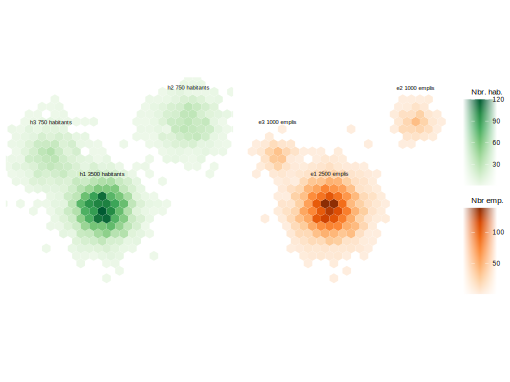
\includegraphics[width=1\textwidth,height=\textheight]{output/gcarte_ss.png}

}

\caption[Territoire synthétique (centre + 2
villages)]{\label{fig-territoire}Territoire synthétique comportant un
centre ville (h1) et deux villages (h2) et (h3). Dans chaque hexagone
est indiqué la densité (5 000 habitants). 4 500 emplois avec des
proportions d'emplois de 80\% dans le centre et de 5\% dans les 2
villages (les 10\% restant sont la fuite). La dispersion est plus basse
pour les emplois. Les densités d'emplois sont représentées dans le
panneau de droite en orange.}

\end{figure}

La figure~\ref{fig-distances} simule \emph{MEAPS} à partir des données
de figure~\ref{fig-territoire}. On obtient pour chaque hexagone de
résident une valeur moyenne de distance jusqu'à leur emploi. De la même
façon, on calcule pour chaque emploi la distance accomplie en moyenne
pour l'atteindre.

\begin{figure}[htb]

{\centering 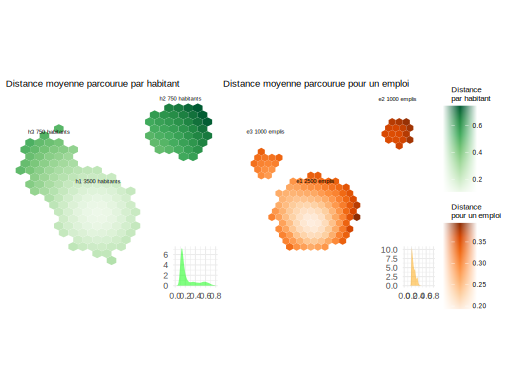
\includegraphics[width=1\textwidth,height=\textheight]{output/gdistances.png}

}

\caption[Distances moyenne par habitant et pour un
emploi]{\label{fig-distances}On représente sur le panneau de
\textbf{gauche} les distances moyennes parcourues par les habitants d'un
héxagone. La vignette présente la densité des trajets en fonction de la
distance(vert). Sur le panneau de \textbf{droite} on représente les
distances moyennes pour atteindre chaque emploi, ainsi que la densité de
ces trajets par distance dans la vignette (orange)}

\end{figure}

Cette première représentation graphique permet de voir le fonctionnement
du modèle \emph{MEAPS}. On peut générer une distribution de trajets
(dans les vignettes de la figure~\ref{fig-distances}). Comme la majorité
des emplois se trouvent dans le pôle central, les distances moyennes
pour les habitants y sont plus faibles que dans les autres pôles. Le
modèle génère un peu de variance à l'intérieur de chaque pôle. On
retrouve l'idée que les hexagones d'habitations les plus excentrées
génèrent des distances plus importantes. La distribution des distances
moyennes pour atteindre un emploi est plus resserrée que celle des
distances parcourues en moyenne par habitant. Les moyennes de ces deux
distributions sont égales (par construction).

On peut construire une table des flux entre chaque pôles
(tableau~\ref{tbl-fluxpoles}). Le premier élément est de noter que les
contraintes aux marges sont parfaitement respectées, ce qui est le
principe de construction de \emph{MEAPS}, les approximations faites dans
l'algorithme de résolution restant ici inférieures à \(10^{-5}\) au
moins. Par ailleurs, la table de flux confirme le diagnostic précédent.
La plupart des habitants de h1 (78\%) se rendent dans g1 (le même pôle
donc). Ce taux d'emploi ``intrapôle'' est de 42\% pour les deux autres
pôles. Ceci tient au déséquilibre de localisation des emplois et est une
propriété souhaitée du modèle. Cela explique en partie la distribution
des distances de la mobilité professionnell pour les habitants et
également sa ``réciproque'', lorsqu'on calcule les distances moyenne
vers un hexagone d'emplois.

\hypertarget{tbl-fluxpoles}{}
\begin{longtable}{lrrrr}
\caption{\label{tbl-fluxpoles}flux entre pôles }\tabularnewline

\toprule
 & e1 & e2 & e3 & total \\ 
\midrule
h1 & 2 481 & 334 & 335 & 3 150 \\ 
h2 & 334 & 290 & 50 & 675 \\ 
h3 & 334 & 51 & 290 & 675 \\ 
total & 3 150 & 675 & 675 & 4 500 \\ 
\bottomrule
\end{longtable}

Pour apprécier le comportement du modèle, on peut procéder à une
expérience de pensée dans laquelle on éloigne les deux pôles satellites
du centre (la distance entre 1 et 2 ou 3 passe de 0.7 à 1.2 dans cette
expérience). Le tableau~\ref{tbl-fluxpoles2} est obtenu en simulant à
nouveau le modèle sur cette géographie alternative. Le résultat est
identique à la configuration précédente. Ce résultat est conforme à
l'intuition et est une propriété souhaitée du modèle. Puisque les ordres
de classement ne changent pas (dès lors que les pôles sont assez
éloignés et que la configuration demeure symétrique), les rangs ne sont
pas modifiés et donc les flux sont inchangés. Les distributions des
distances (sortantes et arrivantes) sont largement modifiées, puisque 2
ou 3 sont plus loin de 1, comme l'indique la
figure~\ref{fig-distances2}. On est tenté de conduire d'autres
expériences de pensée pour analyser le comportement du modèle.
L'application \emph{Shiny} accessible à
\href{https://ofce.shinyapps.io/rmeaps}{ofce.shinyapps.io/rmeaps} permet
de conduire toutes ces expériences en utilisant le même code que celui
utilisé ici.

\hypertarget{tbl-fluxpoles2}{}
\begin{longtable}{lrrrr}
\caption{\label{tbl-fluxpoles2}flux entre pôles (pôle 3 plus loin) }\tabularnewline

\toprule
 & e1 & e2 & e3 & total \\ 
\midrule
h1 & 2 482 & 334 & 334 & 3 150 \\ 
h2 & 334 & 291 & 51 & 675 \\ 
h3 & 334 & 51 & 290 & 675 \\ 
total & 3 150 & 675 & 675 & 4 500 \\ 
\bottomrule
\end{longtable}

\begin{figure}[htb]

{\centering 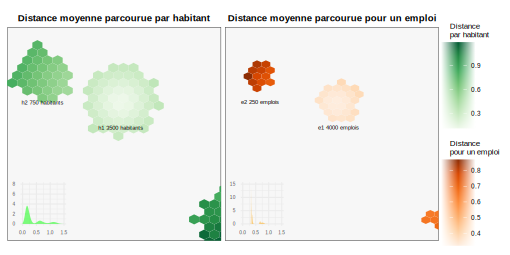
\includegraphics[width=1\textwidth,height=\textheight]{output/gdistances2.png}

}

\caption[Distances moyenne par habitant et pour un emploi (3
éloigné)]{\label{fig-distances2}Le graphique est construit comme le
précédent, le pôle 3 est éloigné de 0.5 (70\% plus loin) par rapport à
1.}

\end{figure}

\begin{figure}[htb]

{\centering \includegraphics[width=1\textwidth,height=\textheight]{output/gdenshabg.png}

}

\caption[Densités comparées]{\label{fig-denscomp}Densités comparées des
distances parcourues par habitant entre le scénario de référence et le
scénario `pôle 3 plus loin'. Le trait pointillé est utilisé pour le
scénario alternatif.}

\end{figure}

\hypertarget{sec-compgravsynth}{%
\section{Comparaison avec le modèle
gravitaire}\label{sec-compgravsynth}}

Comparer \emph{MEAPS} au modèle gravitaire permet d'en comprendre les
avantages. Pour ce faire, nous simulons un modèle gravitaire suivant
l'équation~\ref{eq-gravmod}, c'est-à-dire permettant le calage sur les
lignes (chaque individu a un emploi) et sur les colonnes (chaque emploi
est pourvu). Ce modèle est simulé au niveau désagrégé, c'est-à-dire au
niveau de chaque individu et de chaque emploi à partir de la
configuration géographique décrite plus haut en section~\ref{sec-3p2s}.
La spécification du modèle gravitaire est faite en utilisant comme
fonction \(f\) l'expression suivante où \(\delta\) est un paramètre
positif :

\begin{equation}\protect\hypertarget{eq-f}{}{
f(d) = e^{d/\delta}
}\label{eq-f}\end{equation}

Il s'agit d'un choix très commun. Le modèle gravitaire est ensuite
normalisé en utilisant l'algorithme de Furness (Dios Ortúzar et
Willumsen 2011) dans lequel on normalise d'abord sur les lignes (chaque
individu a un emploi et un seul en probabilité, en tenant compte du
paramètre de fuite), puis sur les colonnes (chaque emploi est pourvu
complètement). On itère ces normalisations en ligne puis en colonne
jusqu'à obtenir une matrice de flux stable. Ces normalisations suivent
les équation~\ref{eq-ai} et équation~\ref{eq-bj}.

Ce modèle gravitaire ainsi spécifié est ajusté sur la simulation
\emph{MEAPS} en prenant comme référence les flux du
tableau~\ref{tbl-fluxpoles}, construits par agrégation sur les groupes
d'habitants et d'emplois -- donc une matrice \(3 \times 3\).
L'ajustement est réalisé en calibrant le paramètre \(\delta\) de façon à
minimiser l'entropie relative de Kullback-Leitner des distributions
agrégées (cette notion d'entropie est détaillée dans la
section~\ref{sec-ajust}). Le résultat de l'estimation est proposé dans
le tableau~\ref{tbl-fluxgrav} et correspond à une valeur de
\(\delta \approx\) 0.53.

\hypertarget{tbl-fluxgrav}{}
\begin{longtable}{lrrrrrlrrrr}
\caption{\label{tbl-fluxgrav}Modèle gravitaire calé sur la configuration de référence }\tabularnewline

\toprule
\multicolumn{5}{c}{MEAPSFuite à 10\%} &  & \multicolumn{5}{c}{GravitaireNormalisé, δ = 0.53} \\ 
\cmidrule(lr){1-5} \cmidrule(lr){7-11}
 & e1 & e2 & e3 & total &   &  & e1 & e2 & e3 & total \\ 
\midrule
h1 & 2 481 & 334 & 335 & 3 150 &  & h1 & 2 953 & 106 & 91 & 3 150 \\ 
h2 & 334 & 290 & 50 & 675 &  & h2 & 533 & 128 & 15 & 675 \\ 
h3 & 334 & 51 & 290 & 675 &  & h3 & 514 & 16 & 144 & 675 \\ 
total & 3 150 & 675 & 675 & 4 500 &  & total & 4 000 & 250 & 250 & 4 500 \\ 
\bottomrule
\end{longtable}

L'ajustement du modèle gravitaire donne un bon résultat. Une des raisons
de ce bon résultat découle de la symétrie de la configuration
géographique. Les deux satellites sont à même distance du pôle central
et la fonction \(f\) qui ne dépend que de la distance permet d'assurer
une répartition des flux entre chacun des pôles sans trop de difficulté.
Si on prend une configuration non symétrique, en éloignant un des deux
satellites, l'autre restant à sa place, on obtient un schéma différent,
le modèle gravitaire amplifiant les asymétries.

\hypertarget{tbl-fluxgrav2}{}
\begin{longtable}{lrrrrrlrrrr}
\caption{\label{tbl-fluxgrav2}Modèle gravitaire pour un satellite éloigné }\tabularnewline

\toprule
\multicolumn{5}{c}{MEAPSFuite à 10\%} &  & \multicolumn{5}{c}{GravitaireNormalisé, δ = 0.53} \\ 
\cmidrule(lr){1-5} \cmidrule(lr){7-11}
 & e1 & e2 & e3 & total &   &  & e1 & e2 & e3 & total \\ 
\midrule
h1 & 2 482 & 334 & 334 & 3 150 &  & h1 & 2 984 & 107 & 59 & 3 150 \\ 
h2 & 334 & 291 & 51 & 675 &  & h2 & 538 & 128 & 9 & 675 \\ 
h3 & 334 & 51 & 290 & 675 &  & h3 & 478 & 15 & 182 & 675 \\ 
total & 3 150 & 675 & 675 & 4 500 &  & total & 4 000 & 250 & 250 & 4 500 \\ 
\bottomrule
\end{longtable}

Le modèle \emph{MEAPS} conserve une configuration identique dans le cas
de pôles satellitaires éloignés du centre, parce que la configuration
reste symétrique et qu'aucun rang n'est modifié. En revanche, le modèle
gravitaire renvoie une réponse très différente de celle du cas de
référence : les habitants des satellites se tournent plus vers les
emplois de leur satellite respectif et les flux entre pôles satellites
et le pôle central se réduisent. Cette propriété du modèle gravitaire
est attendue : la fonction \(f\) donne un poids plus faible aux emplois
plus distants. A la limite où cet éloignement devient particulièrement
grand, les flux entre pôles satellites et le pôle central vont se tarir
presque entièrement. Le paramètre estimé sur la simulation \emph{MEAPS}
est de l'ordre de 0.53, ce qui est l'ordre de grandeur du rayon du pôle
central (0,5). Pour une distance de quelques fois 0.53, les flux entre
pôles seront quasi nul. La réponse de \emph{MEAPS} parait ici plus
adaptée à ce que l'on observe. Lorsque des communes sont satellites d'un
pôle central à une distance de quelques dizaines de kilomètres, il
existe des flux vers cette commune pour occuper des emplois, et le fait
que la commune soit plus éloignée de quelques kilomètres ne tarit pas
drastiquement ces flux. On s'attend à une faible sensibilité de la
distance \emph{à cette échelle}. Nous verrons lors de l'application à
l'agglomération de la Rochelle, en utilisant des données décrivant les
flux entre commune de résidence et commune d'emploi (issues de MOBPRO
(2022)) que \emph{MEAPS} permet une meilleure représentation de la
réalité que le modèle gravitaire.

Si l'on reconduit la procédure d'estimation du paramètre \(\delta\) sur
la configuration géographique où les pôles satellite sont éloignés on
aboutit à \(\delta \approx\) 0.65. Cette valeur est très différente du
paramètre précédent, ce qui montre à la fois la ``plasticité'' du modèle
gravitaire et son manque de fiabilité, comme si la force
``gravitationnelle'' pouvait changer du tout au tout à chaque nouvelle
donnée (tableau~\ref{tbl-fluxgrav3}).

\hypertarget{tbl-fluxgrav3}{}
\begin{longtable}{lrrrrrlrrrr}
\caption{\label{tbl-fluxgrav3}Modèle gravitaire réajusté, satellite éloigné }\tabularnewline

\toprule
\multicolumn{5}{c}{MEAPSFuite à 10\%} &  & \multicolumn{5}{c}{GravitaireNormalisé, δ = 0.65} \\ 
\cmidrule(lr){1-5} \cmidrule(lr){7-11}
 & e1 & e2 & e3 & total &   &  & e1 & e2 & e3 & total \\ 
\midrule
h1 & 2 482 & 334 & 334 & 3 150 &  & h1 & 2 946 & 123 & 81 & 3 150 \\ 
h2 & 334 & 291 & 51 & 675 &  & h2 & 553 & 109 & 13 & 675 \\ 
h3 & 334 & 51 & 290 & 675 &  & h3 & 501 & 18 & 155 & 675 \\ 
total & 3 150 & 675 & 675 & 4 500 &  & total & 4 000 & 250 & 250 & 4 500 \\ 
\bottomrule
\end{longtable}

\hypertarget{sec-estimation}{%
\section{Procédure d'estimation}\label{sec-estimation}}

Il est possible de modifier les pondérations des probabilités
d'absorption de façon à modifier la table des flux. Ceci est illustré
dans la table suivante où on a doublé pour chacune des 9 paires
possibles de zone d'habitation (3) et de zone d'emploi (3) la
probabilité relative d'absorption successivement. La configuration
géographique est celle de la figure~\ref{fig-territoire}, avec un centre
et deux satellites. Le centre comporte plus d'emplois que de résidents,
ce qui oblige à des flux entrants dans la zone 1 comme indiqués dans la-
tableau~\ref{tbl-fluxpoles}. On parle de doublement relatif de la
probabilité, parce que les contraintes de constance de probabilité de
fuite et de saturation des emplois imposent une réduction des
probabilités d'absorption des autres emplois, ce qui est assuré dans
l'algorithme qui implémente \emph{MEAPS}.

Le tableau~\ref{tbl-fluxpond} décrit les variations de flux par rapport
à une situation de référence (celle du tableau~\ref{tbl-fluxpoles}),
arrondi à l'entier le plus proche. Il y a donc \(3 \times 3\) matrices
\(3 \times 3\). Chacune des sous matrices indique les variations de flux
pour chaque paire origine-destination ; il y a 9 possibilités de
doublement de la probabilité d'absorption, qui constituent les lignes et
les colonnes de la matrice englobante. On notera que les sommes des
colonnes et des lignes de chaque sous matrice sont nulles, ce qui
indique le respect des contraintes en ligne et en colonne.

Conformément à l'intuition, et malgré les effets induits par le respect
des contraintes en ligne et en colonne, on observe bien que la paire
zone d'habitation-zone d'emploi qui se voit augmentée en probabilité
relative connait des flux supérieurs. Pour compenser ces flux
supérieurs, dans la même colonne, c'est-à-dire pour les flux en
provenance des autres zones d'habitation, on constate systématiquement
une diminution des flux en provenance des autres zones d'habitation.
Symétriquement, un accroissement des flux de la zone d'habitation \(i\)
vers la zone d'emploi \(j\) induit toujours une diminution des flux de
\(i\) vers les autres zones d'emploi.

\hypertarget{tbl-fluxpond}{}
\setlength{\LTpost}{0mm}
\begin{longtable}{l|lrrrrrrrrr}
\caption{\label{tbl-fluxpond}Modification de la probabilité d'absorption }\tabularnewline

\toprule
\multicolumn{1}{l}{} &  & \multicolumn{3}{c}{e1} & \multicolumn{3}{c}{e2} & \multicolumn{3}{c}{e3} \\ 
\cmidrule(lr){3-5} \cmidrule(lr){6-8} \cmidrule(lr){9-11}
\multicolumn{1}{l}{} &  & e1 & e2 & e3 & e1 & e2 & e3 & e1 & e2 & e3 \\ 
\midrule
h1 & h1 & $76$ & $-38$ & $-38$ & $-72$ & $55$ & $17$ & $-72$ & $17$ & $55$ \\ 
 & h2 & $-38$ & $27$ & $11$ & $81$ & $-63$ & $-18$ & $-9$ & $1$ & $8$ \\ 
 & h3 & $-38$ & $11$ & $27$ & $-9$ & $8$ & $1$ & $81$ & $-18$ & $-63$ \\ 
\midrule
h2 & h1 & $-59$ & $75$ & $-15$ & $75$ & $-76$ & $0$ & $2$ & $-26$ & $24$ \\ 
 & h2 & $51$ & $-58$ & $7$ & $-80$ & $87$ & $-7$ & $7$ & $-12$ & $5$ \\ 
 & h3 & $9$ & $-17$ & $8$ & $5$ & $-12$ & $7$ & $-9$ & $39$ & $-30$ \\ 
\midrule
h3 & h1 & $-59$ & $-15$ & $75$ & $2$ & $24$ & $-26$ & $75$ & $1$ & $-76$ \\ 
 & h2 & $9$ & $8$ & $-17$ & $-9$ & $-30$ & $39$ & $5$ & $7$ & $-11$ \\ 
 & h3 & $51$ & $7$ & $-58$ & $7$ & $5$ & $-13$ & $-80$ & $-7$ & $87$ \\ 
\bottomrule
\end{longtable}
\begin{minipage}{\linewidth}
Le tableau représente l\textquotesingle{}écart entre les flux obtenus pour une probabilité d\textquotesingle{}absorption doublée
pour la zone i d\textquotesingle{}habitation et la zone j d\textquotesingle{}emploi, pour chaque paire de zones habitation/emploi.
La première matrice en haut à gauche indique donc que le flux entre la zone 1 d\textquotesingle{}habitation et
la zone 1 d\textquotesingle{}emploi est accru de 76 lorsque la probabilité d\textquotesingle{}absorption relative est doublée.
Pour compenser ce flux plus important entre 1 et 1, le flux en la zone d\textquotesingle{}habitation 2 et l\textquotesingle{}emploi 1 est réduit de 38,
ce qui implique à son tour que ceux entre 2 et 2 et entre 2 et 3 s\textquotesingle{}accroissent.\\
\end{minipage}

Une propriété intéressante des matrices du tableau~\ref{tbl-fluxpond}
est que les 9 matrices \(3 \times 3\) forment un espace vectoriel de
dimension 4\footnote{Les valeurs propres de la matrice \(9 \times 9\)
  constituée des 9 vecteurs colonnes des 9 matrices ``dérivées'' sont
  (133.3, 97.3, -28.6, 22.0, 0, 0, 0, 0, 0). Les 5 valeurs propres
  nulles et les 4 non nulles permettent de conclure que la dimension de
  l'espace vectoriel engendré par les 9 matrices est 4.}. Ceci est
attendu, puisque les contraintes réduisent la dimension de 9
(\(=3\times 3\)) à 4, puisqu'il y a 3 contraintes dans chaque dimension
(lignes et colonnes) et qu'une est redondante (si les somme sur chaque
ligne sont nulles, alors la somme de tous les coefficients est nulle et
donc si les sommes sur deux colonnes sont nulles, la troisième l'est
nécessairement). Cela indique que, au moins localement (au voisinage de
la matrice de flux calculée dans le tableau~\ref{tbl-fluxpoles}), il est
possible de modifier les probabilités d'absorption pour atteindre
n'importe quelle matrice de flux. A l'approximation linéaire près, il
est donc possible de reproduire n'importe quelle structure de flux
agrégés par un jeu de paramètres saturant exactement la dimension de
cette structure de flux. Cette propriété permet d'envisager différentes
approches d'estimations, suivant les données dont on dispose et du
nombre de degrés de liberté que l'on est prêt à consacrer à la
reproduction des données.

Le temps de calcul peut être assez long du fait de la nécessité de
répéter un grand nombre de tirages, mais la section suivante (
section~\ref{sec-ergemp}) montre que ce nombre peut rester raisonnable.
Une estimation de ce type est mise en oeuvre par une procédure itérative
dans la section Chapitre~\ref{sec-rochelle}, permettant de reproduire à
l'aide de \emph{MEAPS} les données issues de l'enquête mobilités
professionnelles MOBPRO (2022) avec un schéma de calcul qui peut se
mettre facilement en œuvre.

\hypertarget{sec-ergemp}{%
\section{Ergodicité en pratique}\label{sec-ergemp}}

L'utilisation de données synthétiques permet de tester simplement
l'hypothèse d'ergodicité. On a conjecturé que les différentes grandeurs
moyennes sur les permutations \(u\) étaient assimilables à des
observations, éventuellement répétées. A ce stade de simulations
synthétiques nous ne confrontons pas le modèle à des observations (voir
Chapitre~\ref{sec-rochelle}), mais nous allons montrer que l'estimation
des valeurs moyennes ne demande pas l'examen des \(I!\) permutations
possibles\footnote{Par la formule de Stirling
  \(log_{10}(I!) \approx (n +1/2)log_{10} n +log_{10}\sqrt{2} - n log_{10}e \approx 5\times10^5\)
  pour \(I=10^5\), ce qui fait un nombre de grande taille.} et peut se
contenter d'une agrégation spatiale et de quelques tirages de
permutations.

Pour illustrer cette propriété, nous répétons les simulations du modèle
pour plusieurs tirages de priorités (notés \(u\) dans la section
section~\ref{sec-erg}), suivant une méthode de Monte-Carlo. En prenant
la moyenne sur un échantillon de \(u\), on peut construire un estimateur
des grandeurs moyennes et montrer qu'avec un échantillon petit par
rapport à \(I!\), on peut les estimer avec fiabilité et dans un temps
raisonnable. Cette propriété sera montrée sur la structure géographique
particulière que nous avons synthétisée, sans que cela permette de le
généraliser avec certitude. Il existe sans doute des configurations
spatiales pathologiques qui contredisent cette conjecture.

La figure~\ref{fig-emperg} illustre les processus stochastiques à
l'œuvre dans le modèle et leur résolution par la moyennisation sur les
tirages possibles. On applique le modèle en tirant aléatoirement des
permutations de priorité entre les résidents. On représente alors pour
quelques hexagones d'habitation (tirés au sort) l'ensemble des choix de
destination (carroyés dans les hexagones). Le carroyage opère déjà une
moyennisation puisque chacun des individus de chaque hexagone a un ordre
de priorité différent. On représente alors les quantités d'emplois (la
probabilité de choisir un emploi qui se trouve dans l'hexagone
d'arrivée). Les lignes blanches illustrent la dépendance au tirage de
priorité. Mais au bout de quelques tirages, ces probabilités convergent
en moyenne. Pour simuler le modèle, il n'est pas nécessaire (en toute
vraisemblance) de parcourir l'univers complet des permutations.

\begin{figure}[htb]

{\centering \includegraphics[width=1\textwidth,height=\textheight]{output/gemploi_erg.png}

}

\caption[Affectation de l'emploi pour des carreaux de
départ]{\label{fig-emperg}Chaque ligne blanche représente pour un
carreau de départ et d'arrivée (tous les carreaux d'arrivée sont
représenté par une ligne, pour une sélection aléatoire de 4 carreaux de
départ) la probabilité de prendre l'emploi dans le carreau d'arrivée en
fonction du tirage aléatoire. Les lignes vertes représentent cette même
probabibilité prise en moyenne sur les tirages cumulés. L'échelle de
l'axe des y est logarithmique.}

\end{figure}

Le tableau~\ref{tbl-fluxpoles_conf} indique les intervalles de confiance
à 90\% que l'on peut construire à partir des simulations précédentes. On
obtient une stabilité satisfaisante, bien que les flux agrégés soient
stochastiques. Pour une centaine de tirages on peut obtenir une
précision supérieure à \(10^{-3}\).

\hypertarget{tbl-fluxpoles_conf}{}
\setlength{\LTpost}{0mm}
\begin{longtable}{lccc}
\caption{\label{tbl-fluxpoles_conf}flux entre pôles, intervalles de confiance }\tabularnewline

\toprule
 & e1 & e2 & e3 \\ 
\midrule
h1 & 2481{[}2472; 2490{]}ε≈0.1\% & 334{[}329; 339{]}ε≈0.5\% & 335{[}330; 340{]}ε≈0.5\% \\ 
h2 & 334{[}327; 341{]}ε≈0.6\% & 290{[}286; 295{]}ε≈0.5\% & 50{[}49; 52{]}ε≈2\% \\ 
h3 & 334{[}327; 342{]}ε≈0.6\% & 51{[}49; 53{]}ε≈2\% & 290{[}284; 295{]}ε≈0.6\% \\ 
\bottomrule
\end{longtable}
\begin{minipage}{\linewidth}
Source: MEAPS, intervalle à 95\%, 1024 tirages\\
\end{minipage}

Le schéma de saturation et de priorité est illustré par la
figure~\ref{fig-rangerg} ci-dessous. Pour chaque carreau d'arrivée (un
emploi), on représente le rang moyen (gauche) et son écart-type (droite)
au moment de la saturation. La caractère stochastique découle du tirage
aléatoire de l'ordre de chaque individu (les carreaux de départ). Pour
la plupart des emplois, le rang moyen de saturation ergodique est
atteint très rapidement. Les lignes blanches sont rapidement
horizontales, indiquant une rapide convergence du rang moyen au fur et à
mesure que les tirages s'accumulent. Ce graphique confirme qu'à quelques
exceptions près, l'état du système est stable après quelques tirages. Le
panneau de droite illustre l'écart-type observé sur les tirages cumulés.
La nature stochastique du modèle induite par les tirages est ainsi
illustrée.

\begin{figure}[htb]

{\centering \includegraphics[width=1\textwidth,height=\textheight]{output/g_rangns.png}

}

\caption[Rang au moment de la saturation]{\label{fig-rangerg}Chaque
ligne blanche représente pour un carreau d'arrivée (tous les carreaux
d'arrivée sont représenté par une ligne) le rang moyen (panneau gauche)
et l'écart type du rang (panneau de droite).}

\end{figure}

\hypertarget{tension-localisuxe9e-par-emploi}{%
\section{Tension localisée par
emploi}\label{tension-localisuxe9e-par-emploi}}

Le rang moyen au moment de la saturation est une information qui peut
être utilisé pour construire un indicateur localisé de tension comme sur
la figure~\ref{fig-carte_erg}. L'indicateur de tension donne une
information distincte de la distance moyenne ou de la densité de
population ou d'emploi. Les emplois les plus tendus se trouvent sur
l'axe qui relie des pôles. Les emplois situés à la périphérie du pôle
central ont un niveau de tension proche (mais un peu supérieur) à ceux
situés dans les satellites sur la bordure pointant vers le pôle central.
Ces éléments peuvent être utilisés pour identifier les zones pertinentes
de développement de l'emploi.

\begin{figure}[htb]

{\centering \includegraphics[width=1\textwidth,height=\textheight]{output/carte_erg.png}

}

\caption[Indicateur de tension]{\label{fig-carte_erg}Indicateur de
tension relatif localisé égal au rang de saturation normalisé à 100\%
(0\% pour l'emploi saturé le plus tard, 100\% pour l'emploi saturé le
plus tôt, en moyenne sur chaque hexagone d'emploi).}

\end{figure}

L'expérimentation dans l'application \emph{Shiny} permet d'étudier
différentes propriétés de l'indicateur de tension, en particulier
lorsque la tension globale est forte (moins d'emploi que de résidents)
ou faible (excès d'emplois sur les résidents). Dans le cas où il y a un
excès d'emploi sur les résidents, il est possible d'observer une tension
locale sur certains emplois.

\hypertarget{simulation-synthuxe9tiques-dans-shiny}{%
\section{Simulation synthétiques dans
Shiny}\label{simulation-synthuxe9tiques-dans-shiny}}

L'application \href{https://ofce.shinyapps.io./rmeaps/}{shiny rmeaps}
permet de générer des géographies synthétiques et de simuler le modèle
\emph{MEAPS} sur ces distributions. La plupart des graphiques de ce
chapitre peuvent être reproduits de cette façon. L'application permet de
choisir la taille du problème (\(n\) le nombre d'actifs et \(k\) le
nombre d'emploi). En choisissant plus d'emplois que d'actifs on spécifie
un problème où il y a excès d'emplois et donc pas de contrainte globale.
Dans le cas inverse, il y a une fuite, calculée de façon à ce que le
nombre d'actifs restant sur la zone soit égal au nombre d'emplois.

Différents paramètres permettent de spécifier la géographie,
c'est-à-dire la position relative des pôles ou leur taille. Le
simulateur simule par Monte-Carlo plusieurs ordres de passages et
affiche les graphiques correspondants au fur et à mesure de la
convergence, en accumulant la moyenne des différentes variables du
modèle. Cette fonctionnalité permet de visualiser simplement la
propriété d'ergodicité évoquée plus haut.

\bookmarksetup{startatroot}

\hypertarget{sec-rochelle}{%
\chapter{Estimation à La Rochelle}\label{sec-rochelle}}

Nous proposons ici une première application de \emph{MEAPS} à
l'agglomération de la Rochelle. Cette application est issue d'un travail
de quantification de scénarios de politiques publiques visant à réduire
l'empreinte carbone associée aux mobilités quotidiennes et au secteur
résidentiel. La quantification demande à la fois de produire une
cartographie fine des émissions, en procédant par interpolation à partir
de données connues à une maille moins fine et d'être en mesure de
produire des évaluations des différences d'émissions de
CO\textsubscript{2} localement et à l'échelle du territoire selon les
différents scénarios. Nous présentons ici deux familles de scénarios
pour lesquelles \emph{MEAPS} a été mobilisé~:

\begin{itemize}
\item
  Des scénarios de localisation de l'emploi : nous projetons la
  distribution des trajets en utilisant \emph{MEAPS} sur deux structures
  spatiales de l'emploi différentes, tout en conservant la même quantité
  d'emploi globale. La différence entre les kilomètres parcourus suivant
  les différents modes dans les deux scénarios permet d'évaluer l'impact
  de la localisation, en distinguant la contribution du changement
  modal, la contribution des changements de distance pure (à mode et
  flux carreaux à carreaux inchangés) et la contribution des changements
  de flux.
\item
  Des scénarios de modification de la structure du réseau de transport.
  Le principe est identique à celui pour la localisation de l'emploi.
  C'est la matrice des distances et des temps qui est modifiée par une
  modification des infrastructures de transports (par exemple une ligne
  de bus en plus). Cette matrice de distance différente induit des temps
  de trajet plus petits mais uniquement pour le mode transport en
  commun. Elle induit un changement modal (plus de transport en commun,
  moins des autres modes) et enfin conduit à un changement des rangs des
  opportunités et donc une redistribution des flux de carreau à carreau.
\end{itemize}

Dans les deux familles de scénarios, les simulations par \emph{MEAPS}
permettent de construire un contrefactuel et des alternatives à un
niveau fin, croisant la localisation au carreau 200m pour les résidences
(5 456 carreaux pour la Rochelle et le périmètre du SCOT) et les
opportunités (6 326 carreaux dans le périmètre de 33~km autour de
l'agglomération de la Rochelle), soit 34,5 millions de flux et de modes.
L'agrégation de ces informations est alors possible à des niveaux plus
généraux pour analyser les impacts. La conversion des kilomètres ou des
minutes en émissions de CO\textsubscript{2} pour la voiture est
effectuée à partir de coefficients de conversion conventionnels, ce qui
permet d'étendre les indicateurs au champ des émissions de gaz à effet
de serre.

\hypertarget{emplois-ruxe9sidents-au-carreau-inspire-200m}{%
\section{Emplois, résidents au carreau Inspire
200m}\label{emplois-ruxe9sidents-au-carreau-inspire-200m}}

La carte de la zone considérée est représentée sur la
figure~\ref{fig-zoneslr}. L'analyse est limitée aux résidents du
périmètre du Schéma de COhérence Territoriale (SCOT) et considère les
emplois dans un rayon 33 kilomètres autour des lieux de résidence. Cette
carte est construite à partir des données carroyées de C200 (2022) à la
résolution du carreau 200m Inspire\footnote{INfrastructure for SPatial
  InfoRmation in Europe est depuis 2007 une directive pour la production
  de données spatialisées. Inspire définit une grille de carroyage et
  son système de projection harmonisée. C'est ce qui suit l'INSEE dans
  la diffusion des données carroyées. Voir
  https://inspire-geoportal.ec.europa.eu pour la définition de la grille
  et des jeux de données.}. Nous ajoutons à ces données la localisation
de l'emploi sur la même grille en utilisant les fichiers fonciers et les
données d'emplois localisés de MOBPRO (2022). La méthode consiste à
imputer par code NAF les emplois de chaque commune selon MOBPRO (2022)
aux surfaces professionnelles à la parcelle issues des fichiers
fonciers. Cela permet ensuite de localiser au carreau 200m les emplois.
Cette méthode est assez grossière, puisqu'en particulier la ratio
personne/surface n'est pas constant d'une entreprise à l'autre, mais
elle fournit une bonne première approximation d'autant que
l'extrapolation ne dépasse pas l'échelle de la commune. Elle est en tout
cas très supérieure à une imputation uniforme.

\begin{figure}[htb]

{\centering \includegraphics[width=1\textwidth,height=\textheight]{output/popemp.png}

}

\caption[Localisation des résidents et des
emplois]{\label{fig-zoneslr}Localisation des emplois et des résidents,
zones de la Rochelle. Le périmètre de du SCOT de la Rochelle est indiqué
ainsi que les limites administratives des communes et des EPCI le
composant.Sources : OSM, Mapbox, IGN, carroyage INSEE 2017, Flores et
fichiers fonciers 2018}

\end{figure}

\hypertarget{sec-distancesparmode}{%
\section{Calcul des distances par mode}\label{sec-distancesparmode}}

Un ingrédient important de l'analyse du territoire est la prise en
compte des distances entre chaque paire possible résidence/emploi.
Contrairement à l'analyse synthétique, nous ne nous contentons pas de la
distance euclidienne.

Pour ce faire nous calculons à partir d'un calculateur d'itinéraire
(R\textsuperscript{5} de Conveyal (Conway, Byrd, et Linden 2017; Conway,
Byrd, et Van Eggermond 2018; Conway et Stewart 2019) en utilisant le
package \texttt{\{r5r\}} (Pereira et al. 2021) les distances et surtout
les temps de transport pour quatre modes (voiture, vélo, transport en
commun, marche à pied). Les temps de transport calculés pour chaque
paire de carreaux de résidence et d'emploi, en retenant le centre des
carreaux, tiennent compte des différentes contraintes de circulation
(vitesses limites pour la voiture, sens de circulation, pénalité pour
changement de direction, accès autorisé ou restreint suivant le mode,
stress à vélo). Concernant les déplacements en voiture, nous ne prenons
pas en compte à ce stade la congestion. Concernant les transports en
commun, le niveau de détail est assez grand, puisque les fréquences de
circulations des véhicules ainsi que les correspondances sont prises en
compte. Dans certaines villes, il est possible d'accéder à une
information sur les temps de parcours effectifs (mesurant ainsi la
congestion ou la disponibilité du réseau) en complément des horaires
théoriques. Ces informations ne sont pas disponible pour l'agglomération
de la Rochelle et donc cette possibilité n'est pas explorée. L'accès aux
données GTFS impose quelques limites, comme par exemple la non prise en
compte des réseaux scolaires ou d'autres réseaux locaux ou privés non
publiés sous ce format. La modification du réseau de transport comme
l'ouverture d'une ligne ou l'accroissement de fréquence est pris en
compte en modifiant la matrice des distances et temps par mode entre
chaque carreau de résidence et chaque carreau de destination. Dans le
cas de l'agglomération de la Rochelle, le nombre de paires calculés est
de l'ordre de 16 millions.

A partir des temps de trajets par mode, nous appliquons un modèle de
choix discret, \emph{Random Utility Model} (RUM) à la McFadden, estimé
sur l'enquête mobilité des personnes MOBPERS (2021) en utilisant les
données de mobilités professionnelles MOBPRO (2022) pour caler les flux
commune à commune. L'estimation de ce modèle est détaillée dans un autre
document (référence à insérer).

Les distances entre chaque paire de cases permettent de calculer un
indicateur d'accessibilité qui joue un rôle central dans le modèle
radiatif, et donc dans \emph{MEAPS}, en remplaçant la distance par la
somme des opportunités en deçà d'un seuil de temps. Les cartes des
figure~\ref{fig-accto10k} représentent les temps pour accéder à un seuil
d'emplois en utilisant différents modes de transport.

\begin{figure}[htb]

{\centering \includegraphics[width=1\textwidth,height=\textheight]{larochelle_files/figure-pdf/fig-accto10k-1.png}

}

\caption{\label{fig-accto10k}Temps d'accès à 10 000 emplois. Pour chaque
carreau de résidence, on détermine le temps minimal pour atteindre au
moins 10 000 emplois suivant l'un des quatre modes considéré.Calcul des
auteurs. Source : OSM, Mapbox, IGN, Conveyal R5, carroyage INSEE 2017,
Flores et fichiers fonciers 2018}

\end{figure}

Les courbes d'accessibilité de la figure~\ref{fig-comaccess} sont
construites en prenant la moyenne par commune de résidence des temps
d'accès pour les différents seuils d'emplois. C'est cette courbe qui
découle du modèle théorique présenté plus haut (section~\ref{sec-meaps})
et qui détermine les choix individuels de déplacement comme de
localisation. Ces courbes font apparaître une propriété propre aux
villes littorales : si pour des temps courts, l'accès à l'emploi est
maximal à la Rochelle, en revanche d'autres communes jouissent d'une
position plus ``centrale'' lorsqu'on accepte des temps de trajets
supérieurs à 30 minutes en voiture.

\begin{figure}[htb]

{\centering \includegraphics[width=1\textwidth,height=\textheight]{larochelle_files/figure-pdf/fig-comaccess-1.png}

}

\caption[Accessibilité par communes pour la
Rochelle]{\label{fig-comaccess}Courbe du temps d'accès aux emplois. Pour
chaque commune, on calcule la médianne, pondérée par le nombre
d'habitants par carreau, du temps d'accès à différents seuils d'emplois.
Cela permet de caractériser les communes par leur accessibilité à
l'emploi, une mesure plus pertinente de la `distance à l'emploi'. Calcul
des auteurs. Sources : OSM, Mapbox, IGN, Conveyal R5, carroyage INSEE
2017, Flores et fichiers fonciers 2018}

\end{figure}

\hypertarget{sec-ajust}{%
\section{\texorpdfstring{Ajustement de \emph{MEAPS} sur
MOBPRO}{Ajustement de MEAPS sur MOBPRO}}\label{sec-ajust}}

\hypertarget{uxe9miettage-coefficient-dajustement-et-ergodicituxe9}{%
\subsection{émiettage, coefficient d'ajustement et
ergodicité}\label{uxe9miettage-coefficient-dajustement-et-ergodicituxe9}}

La première confrontation empirique peut se faire avec le modèle MEAPS
utilisé tel quel, c'est-à-dire en ne prenant en compte que la fuite.
Pour chaque individu on peut observer dans MOBPRO (2022), par commune de
résidence, un taux de fuite, c'est-à-dire les résidents actifs qui ne
travaillent pas dans le périmètre retenu des communes d'emplois
(figure~\ref{fig-zoneslr}). ce taux de fuite est identique pour tous les
résidents d'une commune, par la résolution spatiale que permet MOBPRO
(2022). En revanche, les informations sur la localisation des emplois et
des résidents ainsi que la structure des distances (mesurées comme le
temps de parcours par mode en utilisant le routage sur les réseaux
disponibles) sont connu à une résolution plus fine. Sur la base de ces
informations, on peut donc simuler à partir de MEAPS des flux entre
carreaux, agrégés entre communes, qui nous servirons de référence.

Dans les simulations synthétiques présentées dans le
Chapitre~\ref{sec-synt} les flux sont simulés avec une granularité
individuelle. Chaque emploi ou chaque individu y est localisé et les
distances sont calculées entre ces localisations et les flux par
individu sont siimulés. L'agrégation spatiale à la maille hexagonale se
fait ensuite. Dans le cas des données que nous utilisons pour La
Rochelle, les carreaux ne sont pas occupés par un seul résident actif ou
un seul emploi. Il y a des paquets pour lesquels il n'est pas nécessaire
de refaire les simulations individu par individu ou emploi par emploi.
Nous les avons donc regroupés et simuler en conséquences dans MEAPS.
Cela pose cependant un problème puisque le choix d'un ordre de priorité
s'exerce maintenant sur des individus en paquets de taille différente,
un faible nombre de ces paquets étant de taille très supérieure à la
médiane des autres. Ainsi, lorsqu'un paquet de taille importante est à
son tour de choisir, il peut saturer des emplois en une seule passe.
Pour résoudre ce problème, nous procédons à un émiettage dans lesquels
les paquets de plus grande taille sont divisés en paquets plus petits.
Pour un seuil d'émiettage de 20 individus (le flux le plus important de
MOBPRO (2022) pour La Rochelle est de 18~000) , on augmente le nombre de
paquets d'environ 50\% ce qui permet de conserver un problème de taille
globale raisonnable tout en réduisant le problème de granularité des
paquets. De plus, les paquets sont tirés au sort dans leur ordre de
priorité en tenant compte de leur taille afin d'éviter une
sur-représentation des paquets de petite taille dans les ordres de
priorité.

Sur la base des flux simulés, on peut définir un critère d'ajustement,
assimilable à un \(R^2\) à partir de l'entropie relative de
Kullback-Leibler (Kullback et Leibler 1951). L'entropie relative est
définie pour deux distributions de probabilités \(p\) et \(q\) comme
suit dans le cas discret :

\[
KL(p,q) = \sum_{i}p_i \times log(p_i/q_i)
\]

Cette mesure ressemble à une distance, mais n'est pas symétrique et ne
vérifie pas l'inégalité triangulaire. Elle s'interprète dans le cadre de
la théorie de l'information comme la quantité relative d'information
supplémentaire nécessaire pour exprimer \(q\) à partir de \(p\). En
suivant Colin Cameron et Windmeijer (1997) on peut construire une mesure
de la qualité de l'ajustement \(R_{KL}^2\) de la façon suivante, où
\(\hat{q}\) et \(q_0\) sont deux distributions, respectivement celles
estimée et de référence, que l'on compare à \(p\) :

\[
R_{KL}^2 = 1 - \frac{KL(p,\hat{q})}{KL(p, q_0)}
\]

La distribution de référence est choisie comme une distribution
uniforme, par analogie avec le calcul de la variance dans un \(R^2\)
habituel où l'on régresse sur une constante. On écrit :

\[
\begin{aligned}
KL(p,q_{ref}) &{}= \sum_{i}p_i \times log(p_i/unif) \\&{}= \sum_i p_i \times log(p_i) + log(N)
\end{aligned}
\]

Ceci n'est autre que l'entropie de la distribution \(p\) à une constante
près (\(N\) est le nombre de résidents actifs ou d'emplois). Le
coefficient d'ajustement ainsi défini peut avoir pour des distributions
particulières des valeurs négatives ou supérieures à 1. Il fonctionne
assez bien malgré tout dans un grand nombre de cas.

Une première évaluation du modèle MEAPS est de comparer ce que l'on
obtient avec MEAPS et un modèle gravitaire simple, estimé sur MOBPRO
(2022), à la maille communale et donc sans recourir à la modélisation
des réseaux de transport décrite plus haut. Le modèle gravitaire estimé
est le suivant, où \(f_{i,j}\) est le flux entre la commune \(i\) de
résidence et la commune \(j\) d'emploi, \(a_i\) sont les actifs en
\$i\$, \(e_j\) l'emploi en \$j\$, et \(t_{i,j}\) le temps de parcours
entre \(i\) et \(j\) en minutes issue des données calculées au carreau
200m agrégés à la maille communale :

\[
log(f_{i,j}) = log(a_i) + log(e_j) - \underset{(7.98)}{0.012} \times t_{i,j} - \underset{(131.7)}{10.02} \\
R^2_{adj} = 2.29\%, 2034\ d.o.f
\]

En ajoutant à la comparaison MEAPS à la maille carreau 200m, on peut
évaluer l'intérêt de la modélisation à la maille infra-communale. La
figure~\ref{fig-divmailles} représente l'ajustement dans les trois
options comparées. Le modèle gravitaire à la maille communale donne un
premier ajustement des données et le \(R^2_{KL}\) est de 77.8\%. MEAPS à
la maille communale donne un résultat moins bon que le modèle
gravitaire, échouant sans plus de paramètres à bien représenter les
flux. Dans ce modèle le \(R^2_{KL}\) est négatif. En revanche, MEAPS
simulé sur le carreau 200m puis agrégé à la maille communale donne un
résultat bien meilleur que les deux précédents modèles. Le \(R^2_{KL}\)
est de 88.4\% et graphiquement l'ajustement apparaît plus satisfaisant.
La seule utilisation des données de réseau et de localisation au carreau
200m permet donc une bien meilleure prédiction de MOBPRO (2022) sans
ajouter de paramètre estimé.

\begin{figure}[htb]

{\centering \includegraphics[width=1\textwidth,height=\textheight]{larochelle_files/figure-pdf/fig-divmailles-1.png}

}

\caption{\label{fig-divmailles}Comparaison de MEAPS et d'un modèle
gravitaire estimé à la maille communale et de MEAPS à la maille carreau
200m}

\end{figure}

La figure~\ref{fig-reflr} représente le \(R^2_{KL}\) que l'on calcule
pour le modèle de référence (MEAPS à la maille carreau 200m) en
effectuant des simulations de Monte-Carlo pour différentes tailles de
l'échantillon d'ordre de priorité. Sans surprise, plus l'échantillon est
grand, plus la distribution des \(R^2_{KL}\) est étroite. Pour 256
tirages, l'intervalle de confiance à 95\% pour le \(R^2_{KL}\) est de
l'ordre de 0.017\% (contre 0.04\% pour 64 tirages et 0.003\% pour 1024
tirages) ce qui sera suffisant pour la plupart des applications.

La valeur moyenne du \(R^2_{KL}\) obtenue pour le MEAPS de référence est
de 88.4\%.

\begin{figure}[htb]

{\centering \includegraphics[width=1\textwidth,height=\textheight]{larochelle_files/figure-pdf/fig-reflr-1.png}

}

\caption{\label{fig-reflr}Densité des \(R^2_{KL}\) simulés par bootstrap
pour une simulation de Monte-Carlo sur 64 ou 256 ou 1024 tirages.}

\end{figure}

\hypertarget{sec-estnp}{%
\subsection{Stratégies d'apprentissage}\label{sec-estnp}}

L'information à la maille carreau 200m est pertinente pour reproduire
les données de MOBPRO (2022). Pour aller plus loin dans l'ajustement,
nous introduisons pour chaque paire (\emph{i}, \emph{j}) un paramètre
qui modifie la probabilité d'absorption de l'individu \emph{i} par
l'emploi \emph{j}. On définit \(c_{abs}\) comme la chance d'absorption,
qui est égale à la probabilité d'être absorbé divisée par la probabilité
de ne pas être absorbée, soit \(c_{abs} = p_{abs}/(1-p_{abs})\) . Dans
le modèle de référence, cette chance d'absorption est similaire pour
tous les emplois considérés par un individu et elle ne dépend que de la
probabilité de fuite. Un moyen simple d'injecter de l'information dans
le modèle consiste alors à modifier cette chance d'absorption selon les
individus et les emplois qu'ils considèrent. Les modifications des
probabilités d'absorption peuvent alors être paramétrées par des
\emph{odds-ratios} (des ratios de chances relatives) \(\omicron_{ij}\)
de telle manière que la nouvelle chance d'absorption de i en j soit
égale à \(\tilde{c}_{abs,ij} = \omicron_{ij} \times c_{abs}\).
L'\emph{odds-ratio} \(\omicron_{ij}\) est un paramètre entre \(0\) et
\(+\infty\) et \emph{i} et \emph{j} indexent les communes de départ et
d'arrivée. La nouvelle probabilité d'absorption s'écrit alors à partir
de la chance d'absorption de référence et de l'\emph{odds-ratio} comme
suit :

\[
\tilde{p}_{abs,ij} = \frac{c_{abs} \times \omicron_{ij}} {1+c_{abs} \times \omicron_{ij}} 
\]

Une première stratégie de calage de \emph{MEAPS} consiste à calculer
autant d'\emph{odds-ratios} qu'il y a de paires communes résidentes -
communes d'emplois de manière à reproduire le plus fidèlement possible
les flux agrégés de MOBPRO (2022). Cette méthode conduit en quelque
sorte à saturer le modèle puisque l'on estime un nombre de paramètres
proche du nombre de degrés de liberté imposé par MOBPRO (2022). Cette
stratégie d'apprentissage est analogue à ce qui se fait en \emph{machine
learning} du fait de la démultiplication du nombre de paramètres à
estimer. La limite de cette approche est le sur-ajustement
(\emph{overfitting}) qu'elle induit. Celle-ci est habituellement
corrigée en ajoutant une pénalité à la complexité du modèle au sein de
la fonction d'optimisation. Cela peut également se faire par
\emph{pruning}, en éliminant \emph{a posteriori} les paramètres dont la
contribution à l'explication des données est inférieure à un seuil.

Les paramètres issues de cette approche contiennent une information qui
peut ensuite être exploitée. Les \emph{odds-ratios} s'interprètent alors
relativement simplement : ceux qui sont supérieurs à 1 indiquent que le
flux de mobilités professionnelles correspondant sont plus fréquents que
ce que prévoit le modèle de référence ; et inversement pour les
\emph{odds-ratios} inférieurs à 1.

Cette approche pose généralement un problème difficile d'optimisation
algorithmique. Une approche brutale, qui consiste à minimiser une
fonction de perte mesurant l'écart entre les flux estimés et les flux
observés, se heurte à la grande dimension de l'espace des paramètres. En
outre, comme toujours dans ce type d'exercice statistique, l'enjeu
consiste à extraire des données disponibles des enseignements généraux
en délaissant ce qui relève de la particularité d'un jeu de données.
C'est toute la difficulté du surapprentissage (\emph{overfitting}) que
nous avons évoquée.

Une seconde approche, plus parcimonieuse, consiste à définir une forme
fonctionnelle pour les \emph{odds-ratios} ou encore à regrouper les
\emph{odds-ratios} en quelques \emph{clusters} pour ensuite n'évaluer
qu'un petit nombre de paramètres. Ceci suppose de modéliser la
structuration des \emph{odds-ratios} à partir d'\emph{a priori} sur les
dimensions pertinentes.

\hypertarget{estimation-de-la-premiuxe8re-approche}{%
\subsection{Estimation de la première
approche}\label{estimation-de-la-premiuxe8re-approche}}

A ce stade, nous utilisons un algorithme naïf pour trouver une solution
au problème posé. Nous calculons les \emph{odds-ratios}
\(\omicron^k_{ij}\) qui permettraient de combler l'écart entre les
prévisions de MEAPS effectuées avec un ensemble d'\emph{odds-ratios}
\(\omicron^{k-1}_{ij}\) et les données observées de MOBPRO (2022) en
utilisant la formule suivante où \(\beta\) est un paramètre
d'amortissement inférieur à 1 et positif et où \(k\) indexe les
itérations :

\begin{equation}\protect\hypertarget{eq-algest}{}{
\omicron^k_{ij} = \biggl(\frac{\tilde{c}^k_{abs}}{
c^{mobpro}_{abs}}\biggr)^\beta \times \omicron^{k-1}_{ij}
}\label{eq-algest}\end{equation}

Nous modifions alors les \(\omicron_{ij}\) en fonction des écarts
observés. Cela conduit à chercher un point fixe.

L'algorithme naïf est relativement efficace. Il converge en quelques
dizaines d'itérations, s'avère stable et fait diminuer l'entropie
relative. Il devra être affiné dans le futur afin de permettre une
descente de gradient qui permet de minimiser explicitement l'entropie
relative. L'algorithme naïf permet de réduire cette entropie relative
sans assurer qu'elle est minimale.

Cet algorithme a été utilisé avec différentes contraintes sur les
paramètres. Le tableau~\ref{tbl-meapsR2-np} indique la qualité de
l'ajustement obtenu dans ces différentes configurations. La première est
celle où les probabilités d'absorption sont déterminées uniquement par
les fuites par commune de résidence. C'est la configuration la plus
parcimonieuse en termes de paramètres et qui sert de référence. Le
\(R^2_{KL}\) vaut 88\% ce qui est un ajustement élevé. La seconde
configuration est celle où l'on ajuste des \(\omicron_{ij}\) uniquement
pour les termes diagonaux (\(i=j\)). Cette configuration ajuste donc un
\emph{odd-ratio} pour les résidents qui travaillent dans leur commune de
résidence. Dans un certain nombre de communes, cet ajustement conduit à
augmenter la probabilité d'absorption interne
(figure~\ref{fig-carteodd}), ce qui indique que le choix de résidence
n'est pas indépendant de celui d'activité. Pour la commune la plus
importante (La Rochelle), en revanche, l'\emph{odd-ratio}
\(\omicron_{17300, 17300}\) est proche de 1. Les deux configurations
suivantes laissent beaucoup plus de degrés de liberté en estimant des
\(\omicron_{ij}\) librement. La première de ces deux configurations
limite les \(\omicron_{ij}\) estimés à ceux représentant un total cumulé
des flux mesurés par MOBPRO (2022) égal à 99.4\%, soit 1~854
\(\omicron_{ij}\) . La seconde configuration estime tous les
\(\omicron_{ij}\) sans limite (soit 2~033 paramètres pour 72 communes de
résidence et 210 communes d'activité, avec un grand nombre de liaisons
non considérées parce que nulles).

\hypertarget{tbl-meapsR2-np}{}
\setlength{\LTpost}{0mm}
\begin{longtable}{lrrr}
\caption{\label{tbl-meapsR2-np}Ajustements non paramètriques, mobilités professionelles la Rochelle }\tabularnewline

\toprule
 & RKL2 & Degrés de liberté & odds estimés \\ 
\midrule
Référence (odds unitiaires) & $88.4\%$ & $1 752$ & $0$ \\ 
Diagonale (résidence égale emploi) & $95.0\%$ & $1 681$ & $71$ \\ 
90\% des flux cumulés & $97.4\%$ & $1 027$ & $725$ \\ 
99\% des flux cumulés  & $99.3\%$ & $0$ & $1 849$ \\ 
100\% des flux cumulés & $99.6\%$ & $0$ & $2 029$ \\ 
\bottomrule
\end{longtable}
\begin{minipage}{\linewidth}
Le nombre de degrés de liberté est le nombre de paires de flux non nuls dans MOBPRO, moins les contraintes en ligne et en colonne, plus un puisqu\textquotesingle{}elles sont redondantes moins le nombre de paramètres estimés. Le nombre de degré de liberté est nul pour les configurations 99\% et 100\% arce que le nombre de paramètres estimés est supérieur au produit des linges et des colonnes moins les contraintes. Il y a bien plus de paramètres estimés pour la configuration 100\%  que pour 99\%. En conséquence, l\textquotesingle{}algorithme conduit à un résultat légèrement différent.\\
\end{minipage}

la figure~\ref{fig-actvsfit-np} représente les flux observés et estimés
pour les différentes configurations du tableau~\ref{tbl-meapsR2-np}. Le
fait d'estimer uniquement les \(\omicron_{ii}\) diagonaux, en ajustant
donc seulement les flux allant d'une commune de résidence vers elle
même, donne déjà de très bons résultats en faisant passer le
\(R^2_{KL}\) de 88\% à 95\% et en réduisant visiblement les écarts entre
flux observé et flux estimé, comme le montrent les deux panneaux
supérieurs de la figure~\ref{fig-actvsfit-np}. L'ajout de paramètres
supplémentaires ne fait pas gagner beaucoup plus, d'autant que les
écarts pour les flux marginaux ne sont pas tant réduits que ça. La
limite de l'algorithme naïf apparaît ici, puisque le modèle complètement
saturé n'ajuste pas totalement la distribution. Différents détails de
l'algorithme peuvent l'expliquer, notamment la censure des
\emph{odd-ratio} trop faibles (\textless0.0001) ou trop importants
(\textgreater10000) ou la prise en compte des flux nuls. Au-delà de cet
argument, il est probable que pour converger vers un ajustement plus
strict, il serait nécessaire de calculer la matrice des quasi dérivées
des flux par rapport aux \(\omicron_{ij}\).

Mais le coût peut être très élevé puisque cette matrice (calculée dans
la partie synthétique dans un cas simple) est d'une taille considérable
(1 755 \(\times\) 1 755 coefficients), surtout si l'on prend en compte
que le calcul de chaque terme prend autour d'une vingtaine de
secondes\footnote{Autour d'une année de vCPU\ldots{}}.

\begin{figure}[htb]

{\centering \includegraphics[width=1\textwidth,height=\textheight]{larochelle_files/figure-pdf/fig-actvsfit-np-1.png}

}

\caption[\emph{MEAPS} observés versus estimés]{\label{fig-actvsfit-np}La
figure présente pour chaque configuration d'estimation le flux observé
(axe des x) et le flux estimé (axe des y) en bleu lorsque oi,j est
estimé et en rouge lorsque oi,j n'est pas estimé (les fuites sont
toujours utilisées). La valeur de référence est répétée dans chaque
panneau en gris clair.}

\end{figure}

Notons que l'échantillon des mobilités donné par MOBPRO (2022) pour
l'agglomération de la Rochelle est très particulier. Une commune (La
Rochelle, dont le code géographique est 17300) représente presque 29\%
des flux de mobilité (de La Rochelle lieu de résidence vers La Rochelle
lieu d'emploi). C'est donc un schéma monocentrique, où à la fois les
résidents et les emplois sont concentrés sur un territoire réduit. La
résolution spatiale de MOBPRO (2022) ne nous permet pas d'en détailler
la structure plus fine.

Pour les 20 plus grandes communes de l'agglomération de la Rochelle --
qui comptent chacune plus de 1 000 résidents en activité -- on peut
représenter les \emph{odds-ratios} estimés dans la configuration 100\%
des flux par rapport aux chances calculées dans le cas où tous les
\(\omicron_{ij}\) sont égaux à 1 (des \emph{odds-ratios} effectifs) en
fonction de la distance entre la commune de destination et la commune de
résidence\footnote{La distance est construite comme la distance moyenne
  pondérée entre les résidents de la commune de départ et les emplois de
  la commune d'arrivée. La pondération est le produit des emplois et des
  résidents pour chaque paire, normalisé à 1.}. Ce diagramme, analogue à
un spectre, peut aussi être construit par commune de destination, la
distance \(d\) étant la distance aux différentes communes de résidence
figure~\ref{fig-spectreE}. L'élément le plus frappant est que les
\emph{odds-ratios} de \(i\) à \(i\) sont généralement supérieur à 1
(figure~\ref{fig-spectreR}), à l'exception de la commune de la Rochelle.
Il n'émerge pas de structure particulière par rapport à la distance, si
ce n'est des \emph{odds-ratios} élevés pour des distances importantes

\begin{figure}[htb]

{\centering \includegraphics[width=1\textwidth,height=\textheight]{output/spectre effectif par COMMUNE 100.png}

}

\caption[Odd-ratio par commune de résidence fonction de la distance aux
communes d'emploi (spectre résidents)]{\label{fig-spectreR}La figure
représente pour les 20 plus grandes communes de l'agglomération de la
Rochelle les odd-ratios estimés (configuration 100\% des flux) en
fonction de la distance entre cette commune et les communes où
travaillent les résidents. Les points marqués d'un petit point blancs
sont les emplois situés hors du périmètre du SCoT.}

\end{figure}

\begin{figure}[htb]

{\centering \includegraphics[width=1\textwidth,height=\textheight]{output/spectre effectif par DCLT 100.png}

}

\caption[Odd-ratio par commune d'emploi fonction de la distance aux
communes de résidence (spectre emplois)]{\label{fig-spectreE}La figure
représente pour les 20 plus grandes communes d'emplois du périmètre
géographique (33 km autour de l'agglomération de la Rochelle) les
odd-ratios estimés (configuration 100\% des flux) en fonction de la
distance entre cette commune et les communes où résident les
travailleurs de la commune.}

\end{figure}

La figure~\ref{fig-carteodd} permet de préciser la valeur élevée des
\emph{odds-ratios} pour les flux internes. Les communes où sont
localisés de nombreux emplois ont un \emph{odds-ratio} plutôt plus
faible alors qu'ils sont estimés plus élevés dans les communes plus
petites et moins desservies. Pour les différentes procédure d'estimation
et donc différents nombres de paramètres estimés, on observe une
structure similaire dans la répartition géographique des
\emph{odds-ratios}, ce qui suggère que les \emph{odds-ratios} estimés
contiennent de l'information.

Un \emph{odds-ratio} élevé dans la diagonale indique que les flux
internes sont plus importants que dans le scénario de référence. Cela
indique probablement un choix de résidence en lien avec l'emploi occupé
en privilégiant la commune d'activité pour résidence (ou éventuellement
l'inverse). Le spectre résident en fonction de la distance indique que
ce phénomène, s'il est une hypothèse à très faible distance, ne persiste
pas en dehors de la commune de résidence. En revanche, la
figure~\ref{fig-spectreE} suggère que dans certaines communes, notamment
Surgères, on observe des \emph{odds-ratios} supérieurs à 1 pour des
distances faibles, ce qui s'interprète comme le fait que les habitants
des communes alentours privilégient Surgères comme lieu d'emploi.

A ce stade, les observations sont limitées par le faible nombre de
communes modélisées, mais on peut espérer que l'analyse des
\emph{odds-ratios} estimés pourra servir à caractériser les communes en
fonction des choix de résidence et d'emploi. En multipliant cette
analyse pour d'autres territoires, l'information apportée par les
\emph{odds-ratios} pourra être inférée. Il sera aussi possible de
confronter ces éléments à d'autres variables, comme le prix de
l'immobilier, les loyers résidentiels ou commerciaux, la densité
d'emploi.

\begin{figure}[htb]

{\centering \includegraphics[width=1\textwidth,height=\textheight]{output/toutes configs odds effectifs.png}

}

\caption[Odd-ratio dans la diagonale]{\label{fig-carteodd}Chaque cercle
indique les odd-ratio estimés dans la diagonale (100\% des flux). Les
diamètres des cercles sont proportionels aux flux internes (de i à i).}

\end{figure}

\hypertarget{estimations-paramuxe9triques-et-comparaison-avec-le-moduxe8le-gravitaire}{%
\subsection{Estimations paramétriques et comparaison avec le modèle
gravitaire}\label{estimations-paramuxe9triques-et-comparaison-avec-le-moduxe8le-gravitaire}}

Au lieu d'estimer directement un ensemble d'\emph{odds-ratios}
\(\omicron_{ij}\), on peut proposer des formes fonctionnelles
paramétriques à partir desquelles on calculera les \emph{odds-ratios}.
C'est une stratégie bien plus parcimonieuse. On détermine alors les
paramètres de la forme fonctionnelle retenue par un algorithme standard
de minimisation de l'entropie relative, qui est le critère que nous
avons choisi pour comparer les distributions. Il est également possible
de conduire une estimation paramétrique pour le modèle gravitaire.

Nous explorons ici trois formes fonctionnelles pour \emph{MEAPS}~:

\begin{enumerate}
\def\labelenumi{\arabic{enumi}.}
\item
  Un paramètre pour tous les termes diagonaux, c'est-à-dire les flux
  allant d'une commune de résidence vers cette même commune pour
  l'emploi. Cette forme est proche de la forme ``diagonale'' estimé dans
  la section~\ref{sec-estnp}, mais un seul paramètre est estimé -- par
  une minimisation de l'entropie relative -- au lieu de 72 par
  l'algorithme itératif. Formellement, \(\omicron_{i \neq j}=1\) et
  \(\omicron_{ii} = o\).
\item
  Un paramètre pour tous les termes diagonaux et un paramètre pour les
  communes voisines d'emploi, c'est-à-dire un terme correctif reliant
  une commune de résidence aux communes voisines. Une commune est
  voisine d'une autre si au moins 5\% des trajets pondérés par les
  emplois et les résidents ont une distance kilométrique inférieure à
  3~km. Cette définition permet d'exclure des communes limitrophes mais
  dont les pôles principaux sont distants. Formellement,
  \(\omicron_{ii} = o_d\); \(\omicron_{ij\in \mathcal{V}(i)} = o_v\) et
  \(\omicron_{i, j \neq i, j \notin \mathcal{V}(i)} = 1\).
\item
  Un coefficient pour la distance et un paramètre pour la distance de
  ``bascule''. Formellement, en dessous d'une distance \(d_c\) , on
  définit un \(\omicron_{ij \in d_{i,j} \leq d_c} = o\) et
  \(\omicron_{ij \in d_{i,j} > d_c} = 1\). Cette forme partage la même
  idée que le premier modèle, mais estime la notion de proximité au lieu
  de reposer sur le découpage administratif.
\end{enumerate}

Chacune de ces options mesure un biais intra-communal qui peut
s'expliquer par un choix conjoint de localisation de résidence et
d'emploi. \emph{MEAPS} offre ici la possibilité de mesurer l'intensité
de ce phénomène par rapport à l'hypothèse où les emplois sont considérés
indépendamment de la localisation et sont tous parfaitement
substituables. Il sera intéressant de comparer les territoires de ce
point de vue et de repérer et quantifier des spécificités locales,
qu'elles concernent la géographie du territoire --~sa structure en pôles
ou en satellite~--, la formation des prix de l'immobilier, le réseau de
transport ou la nature de l'activité économique. On pourrait également
chercher à exploiter l'information sectorielle --~disponible dans MOBPRO
(2022) au niveau de 5 secteurs~-- ou l'information sociale ou
démographique --~disponible au niveau communal ou de l'IRIS mais qui
peut être exploitée également à un niveau plus fin avec
Fidéli\footnote{Fichiers démographiques sur les logements et les
  individus, INSEE,
  https://www.insee.fr/fr/metadonnees/source/serie/s1019.}.

A ces formes fonctionnelles pour \emph{MEAPS}, nous ajoutons deux formes
fonctionnelles pour le modèle gravitaire~:

\begin{enumerate}
\def\labelenumi{\arabic{enumi}.}
\setcounter{enumi}{3}
\tightlist
\item
  un modèle gravitaire suivant la définition équation~\ref{eq-gravity}
  où \(f(d)= e^{d/\delta}\). Un seul paramètre \(\delta\) est estimé.
\item
  un modèle gravitaire ``équilibré'' en utilisant l'algorithme de
  Furness, tel que décrit dans section~\ref{sec-compgravsynth} et en
  estimant \(\delta\) comme dans le point 4.
\end{enumerate}

On pourrait multiplier les modèles estimés\footnote{Par exemple, en
  faisant dépendre les \emph{odd-ratios} non pas de la distance et d'une
  distance critique mais du rang et d'un rang critique.}. Le propos est
ici d'illustrer les possibilités de notre modélisation et de les
comparer à celles du modèle gravitaire. Deux points émergent~:

\begin{itemize}
\item
  \emph{MEAPS} peut mieux reproduire les données, avec une qualité
  d'ajustement meilleure,
\item
  \emph{MEAPS} ouvre des possibilités d'interprétation plus riches que
  celle du modèle gravitaire, parce que les fondements microscopiques de
  \emph{MEAPS} sont explicites.
\end{itemize}

Le tableau tableau~\ref{tbl-meapsR2-p} résume les résultats des
estimations. Le modèle de référence, dans lequel tous les emplois sont
substituables pour chaque individu, fait moins bien en termes
d'ajustement que les autres modèles, à l'exception notable du modèle
gravitaire non équilibré. Comme on avait pu le constater dans les
estimations non paramétriques, le modèle de référence a, malgré son
hypothèse simplificatrice, une bonne performance, ce qui est confirmé
ici par la comparaison au modèle gravitaire simple.

\hypertarget{tbl-meapsR2-p}{}
\setlength{\LTpost}{0mm}
\begin{longtable}{lccc}
\caption{\label{tbl-meapsR2-p}Ajustements paramètriques, mobilités professionelles la Rochelle }\tabularnewline

\toprule
 & RKL2 & Degrés de liberté & Paramètres \\ 
\midrule
 Référence & $88.4\%$ & $1 752$ &  \\ 
1. Commune vers commune & $93.0\%$ & $1 751$ & NA \\ 
2. Commune vers commune et voisines & $93.1\%$ & $1 750$ & od≈4.3 ov≈1.3 \\ 
3. Distance carreau 200m & $94.1\%$ & $1 750$ & dc≈ 9 min o≈19 \\ 
4. Gravitaire sans Furness & $82.6\%$ & $1 961$ & δ≈20 min \\ 
5. Gravitaire avec Furness & $90.7\%$ & $1 751$ & δ≈17 min \\ 
\bottomrule
\end{longtable}
\begin{minipage}{\linewidth}
Le nombre de degrés de liberté est le nombre de paires de flux non nuls dans MOBPRO, moins les contraintes en ligne et en colonne, plus un puisqu\textquotesingle{}elles sont redondantes moins le nombre de paramètres estimés. Les unités sont des minutes de trajet pour les paramètres homogènes à une distance et sans unité pour les \emph{odd-ratios}.\\
\end{minipage}

Les estimations des modèles 1 à 3, dans lesquelles on explore un terme
diagonal sous différentes formes, renforcent le diagnostic de biais
communal noté dans les estimations non paramétriques. Il y a en moyenne
4 fois plus de chance de choisir un emploi (tableau~\ref{tbl-meapsR2-p},
lignes 1 et 2) dans la commune de résidence. L'estimation du modèle 2
montre que les communes voisines ne connaissent pas un biais comparable,
bien que la chance de choisir un emploi dans celles-ci soit supérieure à
1.

L'estimation du modèle 3 indique qu'apparemment la distance explique
mieux le biais communal que le découpage administratif et il convient
plutôt de voir celui-ci comme un biais de proximité. En effet, le
coefficient d'ajustement est supérieur de plus d'un point à celui obtenu
avec le premier modèle, en perdant uniquement 1 degré de liberté. La
distance de bascule est faible, autour de 9 minutes, ce qui suggère que
le périmètre communal est trop large pour capturer cet effet. La chance
à plus courte distance est également nettement plus élevée puisqu'au
lieu d'être approximativement de 4 elle est approximativement de 19,
soit plus de 4 fois plus.

Il convient à ce stade d'être prudent sur cette estimation, puisque la
résolution des données est largement inférieure au seuil qui a été
trouvé. La simulation est basée sur des distances et des localisations
d'emplois au carreau 200m dont la précision est convaincante. Mais les
flux dans MOBPRO (2022) ne sont connus que pour les communes d'origine
et de départ et donc avec une résolution spatiale plus faible. La
multiplication des observations peut palier à cette faible résolution
spatiale, mais cela demandera d'établir une analyse des distances et des
localisations sur des territoires plus grands et plus nombreux. Pour
avancer, il faudrait recourir à des données de flux plus finement
localisées, par exemple à partir de Fidéli\footnote{A partir de Fidéli,
  on peut préciser la localisation de chaque individu et utiliser
  l'information sur la commune dans laquelle il travaille. On ne peut
  pas en revanche localiser plus précisément la localisation de l'emploi
  occupé.} ou de données issues de traçages numériques.

\begin{figure}[htb]

{\centering \includegraphics[width=1\textwidth,height=\textheight]{larochelle_files/figure-pdf/fig-actvsfit-p-1.png}

}

\caption[\emph{MEAPS} observés versus estimés, estimations
paramétriques]{\label{fig-actvsfit-p}La figure présente pour chaque
configuration d'estimation le flux observé (axe des x) et le flux estimé
(axe des y) en bleu lorsque oi,j est estimé et en rouge lorsque oi,j
n'est pas estimé (les fuites sont toujours utilisées). La valeur de
référence est répétée dans chaque panneau en gris clair.}

\end{figure}

Les estimations paramétriques indiquent une moins bonne performance du
modèle gravitaire. Sans respect des contraintes en colonne, le modèle
gravitaire donne une image assez faussée des trajets. Il peine à
reproduire le biais de proximité et l'influence de la distance. Le
premier tend à produire un paramètre \(\delta\) très élevé alors que le
second devrait au contraire imposer un \(\delta\) plus faible pour
rendre compte de trajets plus longs. L'application d'une même valeur de
la distance suivant des milieux plus ou moins denses handicape cette
représentation. La procédure de Furness améliore la capacité du modèle
gravitaire à rendre compte des données, mais, comme nous le disions, au
prix de la perte du lien avec la distance telle qu'elle est formulée
dans le modèle gravitaire, à savoir homogène pour tous.

La figure~\ref{fig-actvsfit-grav} illustre ce qui est à l'œuvre dans le
modèle gravitaire. La minimisation de l'entropie relative dépend
beaucoup des flux à l'intérieur de La Rochelle, qui pèsent 29\% de
l'échantillon. La prise en compte des autres communes diagonales n'est
pas bonne, ce qui conduit à un \(R^2_{KL}\) moins bons que la référence
de \emph{MEAPS} (tous les emplois sont identiques pour chaque individu
et ne diffèrent que par leur localisation). Le respect de la contrainte
en colonne par la procédure de Furness permet une meilleure prise en
compte des communes diagonales (dont le poids est de 35\% dans
l'échantillon La Rochelle), mais moins bonne que les modèles
\emph{MEAPS} paramétriques ou non.

\begin{figure}[htb]

{\centering \includegraphics[width=1\textwidth,height=\textheight]{larochelle_files/figure-pdf/fig-actvsfit-grav-1.png}

}

\caption[\emph{MEAPS} observés versus
estimés]{\label{fig-actvsfit-grav}La figure présente pour chaque
configuration d'estimation le flux observé (axe des x) et le flux estimé
(axe des y) en bleu lorsque oi,j est estimé et en rouge lorsque oi,j
n'est pas estimé (les fuites sont toujours utilisées). La valeur de
référence est répétée dans chaque panneau en gris clair.}

\end{figure}

La figure~\ref{fig-distrdist} confirme ce diagnostic. On y compare la
distrbution cumulée en fonction de la distance kilométrique pondérée
entre chaque commune pour différentes estimations, les flux de MOBPRO
(2022) étant utilisé comme référence. Les performances des modèles sont
comparables pour les courtes distances (i.e la commune de la Rochelle
vers elle-même). Le modèle gravitaire avec ou sans Furness pêche sur les
distances intermédiaires et donne trop de poids aux distances très
longues. Les estimations paramétriques à partir de \emph{MEAPS}
parviennent bien à reproduire la distribution cumulée des distances,
notamment le modèle paramétrique 3. qui retient la distance au carreau
200m comme forme fonctionnelle.

\begin{figure}[htb]

{\centering \includegraphics[width=1\textwidth,height=\textheight]{larochelle_files/figure-pdf/fig-distrdist-1.png}

}

\caption[Distributions empiriques cumulées des
distances]{\label{fig-distrdist}Distributions empiriques cumulées des
flux selon la distance. MOBPRO est indiqué en trait pointillé noir. La
figure du haut est la distribution cumulée, celle du bas la différence
entre la distribution et celle de MOBPRO}

\end{figure}

\hypertarget{une-cartographie-des-uxe9missions-de-co2}{%
\section{\texorpdfstring{Une cartographie des émissions de
CO\textsubscript{2}}{Une cartographie des émissions de CO2}}\label{une-cartographie-des-uxe9missions-de-co2}}

La construction d'un modèle et sa calibration et sa validation sur des
données permet de projeter dans des dimensions non observées les
prédictions du modèle. Nous utilisons ici \emph{MEAPS}, calibré sur les
données MOBPRO (2022) sur l'agglomération de la Rochelle pour produire
une carte au carreau 200m des émissions de CO\textsubscript{2} liées à
la mobilité professionnelle quotidienne.

Le principe est assez simple : les seuls déplacements en voiture sont
considérés comme étant émetteur de CO\textsubscript{2}, ce qui est une
approximation raisonnable. Les émissions liées aux transports en commun,
particulièrement les bus peu occupés pourraient être ajoutées, mais
elles pèsent relativement peu dans le bilan des mobilités quotidiennes.
Pour estimer les déplacements en voiture nous utilisons un modèle de
choix discret évoqué dans la section~\ref{sec-distancesparmode}. Ce
modèle estimé sur MOBPERS (2021) ne pose à ce stade pas de difficulté
particulière, si ce n'est un problème discuté à la fin de cette section.

\bookmarksetup{startatroot}

\hypertarget{sec-scenarios}{%
\chapter{Scénarios à la Rochelle}\label{sec-scenarios}}

La construction d'un modèle représentant de façon fine et fiable les
déplacements permet de proposer des analyses pour des scénarios
complexes. C'est le but d'une modélisation que de proposer des réposnes
convaincantes à des questions du type ``Que se passerait-il
si\ldots{}''. Dans la réponse à une telle question, on esp\^{}ère que la
modélisation permet de la prendre en compte avec une profondeur
suffisante et que les éléments calibrés sur les observations sont
suffisamment invariants pour justifier une projection.

\hypertarget{re-localisation-de-lemploi}{%
\section{Re-localisation de l'emploi}\label{re-localisation-de-lemploi}}

Le Schéma de Cohérence Territorial (SCoT) est un document de
planification, établi et voté par les élus des communes composant le
territoire et soumis à validation de l'État. Il défini, entre autres,
des zones de développement économique, urbaines et des espaces naturels.
C'est la loi SRU relative à la Solidarité et au Renouvellement Urbains
du 13 décembre 2000 qui l'a défini et les contours en ont été modifiés
au cours des dernières années.

Le schéma n'est pas qu'indicatif puisqu'il est opposable. En ce qui
concerne le développement de l'emploi, la création de zones d'activité
est rendue possible par le SCoT, mais la réalisation effective des
créations d'emploi et surtout leur localisation nette des déplacements
d'autres emplois découle des décisions de l'ensemble des acteurs et donc
et donc de causalités diverses et variées. Nous évaluons ici des
scénarios comptatibles avec le SCoT sans pour autant nous prononcer
quant à leur réalisme ou leur probabilité d'occurrence. Ainsi, nous
analysons les localisations proposées à emploi total constant,
c'est-à-dire vues comme des relocalisations de l'emploi vers les zones
d'activités depuis leur localisation actuelle.

\hypertarget{reconfiguration-du-ruxe9seau-de-transport-en-commun}{%
\section{Reconfiguration du réseau de transport en
commun}\label{reconfiguration-du-ruxe9seau-de-transport-en-commun}}

L'analyse du territoire ne repose pas seulement sur la localisation de
l'emploi, mais aussi sur une prise en compte détaillée des possibilités
de transport.

\bookmarksetup{startatroot}

\hypertarget{ruxe9fuxe9rences}{%
\chapter*{Références}\label{ruxe9fuxe9rences}}
\addcontentsline{toc}{chapter}{Références}

\markboth{Références}{Références}

\hypertarget{refs}{}
\begin{CSLReferences}{1}{0}
\leavevmode\vadjust pre{\hypertarget{ref-ben-akiva2018}{}}%
Ben-Akiva, Moshe, et Steven R. Lerman. 2018. \emph{Discrete Choice
Analysis: Theory and Application to Travel Demand}. Transportation
Series. MIT Press.

\leavevmode\vadjust pre{\hypertarget{ref-C200}{}}%
C200. 2022. {«~Revenus, pauvreté et niveau de vie en 2017 - Données
carroyées. Dispositif Fichier localisé social et fiscal (Filosofi)~»}.
INSEE;
\url{https://www.insee.fr/fr/statistiques/6214811?sommaire=6215217}.

\leavevmode\vadjust pre{\hypertarget{ref-colincameron1997}{}}%
Colin Cameron, A., et Frank A. G. Windmeijer. 1997. {«~An R-Squared
Measure of Goodness of Fit for Some Common Nonlinear Regression
Models~»}. \emph{Journal of Econometrics} 77 (2): 329‑42.
\url{https://doi.org/10.1016/s0304-4076(96)01818-0}.

\leavevmode\vadjust pre{\hypertarget{ref-conway2017}{}}%
Conway, Matthew Wigginton, Andrew Byrd, et Marco van der Linden. 2017.
{«~Evidence-Based Transit and Land Use Sketch Planning Using Interactive
Accessibility Methods on Combined Schedule and Headway-Based
Networks~»}. \emph{Transportation Research Record: Journal of the
Transportation Research Board} 2653 (1): 45‑53.
\url{https://doi.org/10.3141/2653-06}.

\leavevmode\vadjust pre{\hypertarget{ref-conway2018}{}}%
Conway, Matthew Wigginton, Andrew Byrd, et Michael Van Eggermond. 2018.
{«~Accounting for uncertainty and variation in accessibility metrics for
public transport sketch planning~»}. \emph{Journal of Transport and Land
Use} 11 (1). \url{https://doi.org/10.5198/jtlu.2018.1074}.

\leavevmode\vadjust pre{\hypertarget{ref-conway2019}{}}%
Conway, Matthew Wigginton, et Anson F. Stewart. 2019. {«~Getting Charlie
Off the MTA: A Multiobjective Optimization Method to Account for Cost
Constraints in Public Transit Accessibility Metrics~»}.
\emph{International Journal of Geographical Information Science} 33 (9):
1759‑87. \url{https://doi.org/10.1080/13658816.2019.1605075}.

\leavevmode\vadjust pre{\hypertarget{ref-de2011modelling}{}}%
Dios Ortúzar, Juan de, et Luis G Willumsen. 2011. \emph{Modelling
transport}. John wiley \& sons.

\leavevmode\vadjust pre{\hypertarget{ref-heanue1966}{}}%
Heanue, Kevin E., et Clyde E. Pyers. 1966. {«~A Comparative Evaluation
of Trip Distribution Procedures~»}. \emph{Highway Reserach Record}, nᵒ
114: 20‑50.

\leavevmode\vadjust pre{\hypertarget{ref-kullback1951}{}}%
Kullback, S., et R. A. Leibler. 1951. {«~On Information and
Sufficiency~»}. \emph{The Annals of Mathematical Statistics} 22 (1):
79‑86. \url{https://doi.org/10.1214/aoms/1177729694}.

\leavevmode\vadjust pre{\hypertarget{ref-lasser2020}{}}%
Lasser, Jana. 2020. {«~Creating an Executable Paper Is a Journey Through
Open Science~»}. \emph{Communications Physics} 3 (1).
\url{https://doi.org/10.1038/s42005-020-00403-4}.

\leavevmode\vadjust pre{\hypertarget{ref-MOBPERS}{}}%
MOBPERS. 2021. {«~EMP 2019 Résultats détaillés de l'enquête mobilité des
personnes de 2019~»}. SDES, Ministère de la transition écologique et de
la cohésion des territoires;
\url{https://www.statistiques.developpement-durable.gouv.fr/resultats-detailles-de-lenquete-mobilite-des-personnes-de-2019}.

\leavevmode\vadjust pre{\hypertarget{ref-MOBPRO}{}}%
MOBPRO. 2022. {«~Mobilités professionnelles en 2019 : déplacements
domicile - lieu de travail Recensement de la population - Base flux de
mobilité~»}. INSEE; \url{https://www.insee.fr/fr/statistiques/6454112}.

\leavevmode\vadjust pre{\hypertarget{ref-patrickbonnel2001}{}}%
Patrick Bonnel. 2001. {«~Prévision de la demande de transport~»}. Thèse
de doctorat, Lyon, France.

\leavevmode\vadjust pre{\hypertarget{ref-r5r}{}}%
Pereira, Rafael H. M., Marcus Saraiva, Daniel Herszenhut, Carlos Kaue
Vieira Braga, et Matthew Wigginton Conway. 2021. {«~r5r: Rapid Realistic
Routing on Multimodal Transport Networks with R5 in R~»}.
\url{https://doi.org/10.32866/001c.21262}.

\leavevmode\vadjust pre{\hypertarget{ref-simini2012}{}}%
Simini, Filippo, Marta C. González, Amos Maritan, et Albert-László
Barabási. 2012. {«~A Universal Model for Mobility and Migration
Patterns~»}. \emph{Nature} 484 (7392): 96‑100.
\url{https://doi.org/10.1038/nature10856}.

\leavevmode\vadjust pre{\hypertarget{ref-stouffer1940}{}}%
Stouffer, Samuel A. 1940. {«~Intervening Opportunities: A Theory
Relating Mobility and Distance~»}. \emph{American Sociological Review} 5
(6): 845. \url{https://doi.org/10.2307/2084520}.

\leavevmode\vadjust pre{\hypertarget{ref-wilson1967}{}}%
Wilson, A. G. 1967. {«~A Statistical Theory of Spatial Distribution
Models~»}. \emph{Transportation Research} 1 (3): 253‑69.
\url{https://doi.org/10.1016/0041-1647(67)90035-4}.

\end{CSLReferences}



\end{document}
